\documentclass[]{article}
\usepackage{lmodern}
\usepackage{amssymb,amsmath}
\usepackage{ifxetex,ifluatex}
\usepackage{fixltx2e} % provides \textsubscript
\ifnum 0\ifxetex 1\fi\ifluatex 1\fi=0 % if pdftex
  \usepackage[T1]{fontenc}
  \usepackage[utf8]{inputenc}
\else % if luatex or xelatex
  \ifxetex
    \usepackage{mathspec}
    \usepackage{xltxtra,xunicode}
  \else
    \usepackage{fontspec}
  \fi
  \defaultfontfeatures{Mapping=tex-text,Scale=MatchLowercase}
  \newcommand{\euro}{€}
\fi
% use upquote if available, for straight quotes in verbatim environments
\IfFileExists{upquote.sty}{\usepackage{upquote}}{}
% use microtype if available
\IfFileExists{microtype.sty}{%
\usepackage{microtype}
\UseMicrotypeSet[protrusion]{basicmath} % disable protrusion for tt fonts
}{}
\usepackage{graphicx}
\makeatletter
\def\maxwidth{\ifdim\Gin@nat@width>\linewidth\linewidth\else\Gin@nat@width\fi}
\def\maxheight{\ifdim\Gin@nat@height>\textheight\textheight\else\Gin@nat@height\fi}
\makeatother
% Scale images if necessary, so that they will not overflow the page
% margins by default, and it is still possible to overwrite the defaults
% using explicit options in \includegraphics[width, height, ...]{}
\setkeys{Gin}{width=\maxwidth,height=\maxheight,keepaspectratio}
\ifxetex
  \usepackage[setpagesize=false, % page size defined by xetex
              unicode=false, % unicode breaks when used with xetex
              xetex]{hyperref}
\else
  \usepackage[unicode=true]{hyperref}
\fi
\hypersetup{breaklinks=true,
            bookmarks=true,
            pdfauthor={Guillermo Jiménez Díaz (gjimenez@ucm.es); Alberto Díaz (albertodiaz@fdi.ucm.es)},
            pdftitle={Análisis de Redes Sociales},
            colorlinks=true,
            citecolor=blue,
            urlcolor=blue,
            linkcolor=magenta,
            pdfborder={0 0 0}}
\urlstyle{same}  % don't use monospace font for urls
\setlength{\parindent}{0pt}
\setlength{\parskip}{6pt plus 2pt minus 1pt}
\setlength{\emergencystretch}{3em}  % prevent overfull lines
\setcounter{secnumdepth}{5}

\title{Análisis de Redes Sociales}
\author{Guillermo Jiménez Díaz (gjimenez@ucm.es) \and Alberto Díaz (albertodiaz@fdi.ucm.es)}
\date{5 de diciembre de 2014}

\begin{document}
\maketitle

\section*{Prefacio}\label{prefacio}
\addcontentsline{toc}{section}{Prefacio}

Estos son los apuntes de la asignatura Análisis de Redes Sociales,
impartida en la Facultad de Informática de la Universidad Complutense de
Madrid por los profesores Guillermo Jiménez Díaz y Alberto Díaz, del
Departamento de Ingeniería del Software e Inteligencia Artificial.

Este material ha sido desarrollado a partir de distintas fuertes,
destacando como referencia principal el libro \emph{Network Science} de
Laszlo Barabasi, el material de la asignatura \emph{Social Network
Analysis}, impartido por Lada Adamic a través de Coursera, y las
transparencias de la asignatura Redes y Sistemas Complejos, creadas por
Óscar Cordón García de la Universidad de Granada.

Para este capítulo se ha utilizado, adicionalmente, material de los
libros \emph{Analyzing the Social Web} de Jennifer Goldbeck (capítulo
10) y \emph{Networks, Crowds, and Markets} de Easley y Kleinberg
(capítulos 19 y 21).

Este obra está bajo una
\href{http://creativecommons.org/licenses/by-nc-sa/4.0/}{licencia de
Creative Commons Reconocimiento-NoComercial-CompartirIgual 4.0
Internacional}.

\setcounter{section}{8}

\section*{Tema 8: Propagación y Difusión en
redes}\label{tema-8-propagaciuxf3n-y-difusiuxf3n-en-redes}
\addcontentsline{toc}{section}{Tema 8: Propagación y Difusión en redes}

Las conexiones presentes en la redes permiten modelar la propagación de
todo tipo de elementos entre sus nodos: enfermedades, vídeos virales,
rumores, virus informáticos, productos, anuncios, información\ldots{} En
general, la mayoría de estos modelos de propagación son similares
independientemente de lo que se pretenda propagar.

Existe desde hace muchos años un estudio intenso en la propagación de
enfermedades. El conocimiento de cómo se propagan a través de una red de
individuos nos puede servir para entender cómo se puede propagar
cualquier otro tipo de información en dicha red. Por este motivo, en
este tema vamos a hablar los modelos fundamentales de propagación de
enfermedades y vamos a estudiar como aplicarlos a las redes, analizando
cómo la estructura de la misma afecta enormemente a estos fenómenos de
propagación.

\subsection{Modelos de contagio
simple}\label{modelos-de-contagio-simple}

La epidemiología es la ciencia que estudia la salud y control de
enfermedades en una población, así como la predicción de expansión de
dichas enfermedades. El modelo general epidemiológico se basa en dos
hipótesis:

\begin{itemize}
\itemsep1pt\parskip0pt\parsep0pt
\item
  \textbf{Modelo compartimental}: cada individuo puede estar en un
  determinado estado dependiendo de en qué fase se la enfermedad se
  encuentra. El modelo más simple, que será el que usemos, supone 3
  estados:

  \begin{itemize}
  \itemsep1pt\parskip0pt\parsep0pt
  \item
    \textbf{Susceptible (S)}: El individuo está sano y puede ser
    infectado.
  \item
    \textbf{Infectado (I)}: El individuo está infectado y puede
    contagiar a otros individuos.
  \item
    \textbf{Recuperado (R)}: El individuo estuvo contagiado pero se ha
    recuperado y no puede volver a ser contagiado. También se utiliza
    para modelar los individuos que no han superado la enfermedad y que
    han muerto a causa de ella.
  \end{itemize}
\item
  \textbf{Mezcla homogénea}: Cualquier individuo tiene la misma
  probabilidad de estar en contacto con un individuo infectado. Esta
  hipótesis puede interpretarse como que la red de contactos está
  modelada mediante una red aleatoria aunque, realmente, elimina la
  necesidad de conocer los contactos de los individuos y se puede asumir
  que cualquiera puede infectar a cualquiera.
\end{itemize}

Los modelos generados a partir de estas hipótesis observan el
comportamiento (los cambios de estado) de los individuos a lo largo del
tiempo para predecir el alcance y la velocidad de propagación de la
enfermedad, entre otras. A continuación vamos a estudiar la dinámica de
los modelos de propagación clásicos, que combinan las letras del modelo
compartimental.

\subsubsection{Modelo SI}\label{modelo-si}

Es el modelo más sencillo, en el que un individuo susceptible puede
quedar infectado pero, una vez infectado, no se puede recuperar. Un
ejemplo de este tipo es el virus del VIH (o los zombies).

\begin{figure}[htbp]
\centering
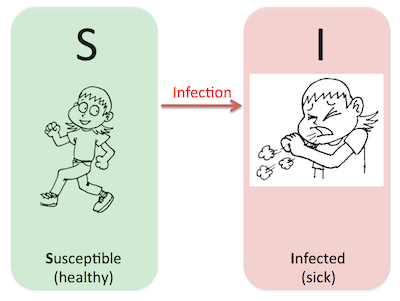
\includegraphics{../images/tema08/modeloSI.png}
\caption{Esquema del Modelo SI}
\end{figure}

En este modelo suponemos que cada individuo tiene \(\langle k \rangle\)
contactos (enlaces) y que en cada instante de tiempo la enfermedad se
propaga con una tasa de contagio \(\delta\), que representa la
probabilidad de que un individuo infectado transmita la enfermedad a uno
susceptible.

Para entender la dinámica del modelo vamos a definir los siguientes
parámetros.

\begin{itemize}
\itemsep1pt\parskip0pt\parsep0pt
\item
  \(N\) es el tamaño de la población y es \(N = S(t) + I(t)\), donde
  \(S(t)\) (número de individuos que están en el estado susceptible en
  el tiempo \(t\)) e \(I(t)\) (número de individuos que están en el
  estado infectado en el tiempo \(t\)).
\item
  En lugar de manejar valores absolutos vamos a manejar las proporciones
  o ratios de susceptibles e infectados. De este modo
  \(s(t) = s = \frac{S(t)}{N}\) representa la proporción de individuos
  susceptibles de la población mientras que
  \(i(t) = i = \frac{I(t)}{N}\).
\item
  \(\beta\) es la tasa de transmisión que incluye el grado medio de cada
  individuo, esto es, \(\beta = \delta \cdot \langle k \rangle\).
\end{itemize}

La ecuación diferencial que modela la tasa a la que varía el número de
infectados es:

\[\frac{di}{dt} = i \cdot \beta  \cdot s = i \cdot \beta \cdot (1-i)\]

En cada momento de tiempo, la proporción de infectados es la cantidad de
infectados \(i\) más la proporción de individuos susceptibles que pueden
ser infectados \(\beta \cdot s\).

Si resolvemos esta ecuación nos queda que:

\[i = \frac{i_0exp(\beta t)}{1-i_0+i_0exp(\beta t)}\]

donde \(i_0\) representa a la tasa de infectados en el instante \(t=0\).
De la representación gráfica de esta función extraemos las siguientes
conclusiones:

\begin{itemize}
\itemsep1pt\parskip0pt\parsep0pt
\item
  Inicialmente el número de infectados crece exponencialmente.
\item
  A medida que el número de infectados se hace mayor, hay menos
  individuos susceptibles por lo que el crecimiento de infectados se
  ralentiza y la infección termina cuando todos están infectados
  (\(i(t \to \infty)= 1\)).
\end{itemize}

\begin{figure}[htbp]
\centering
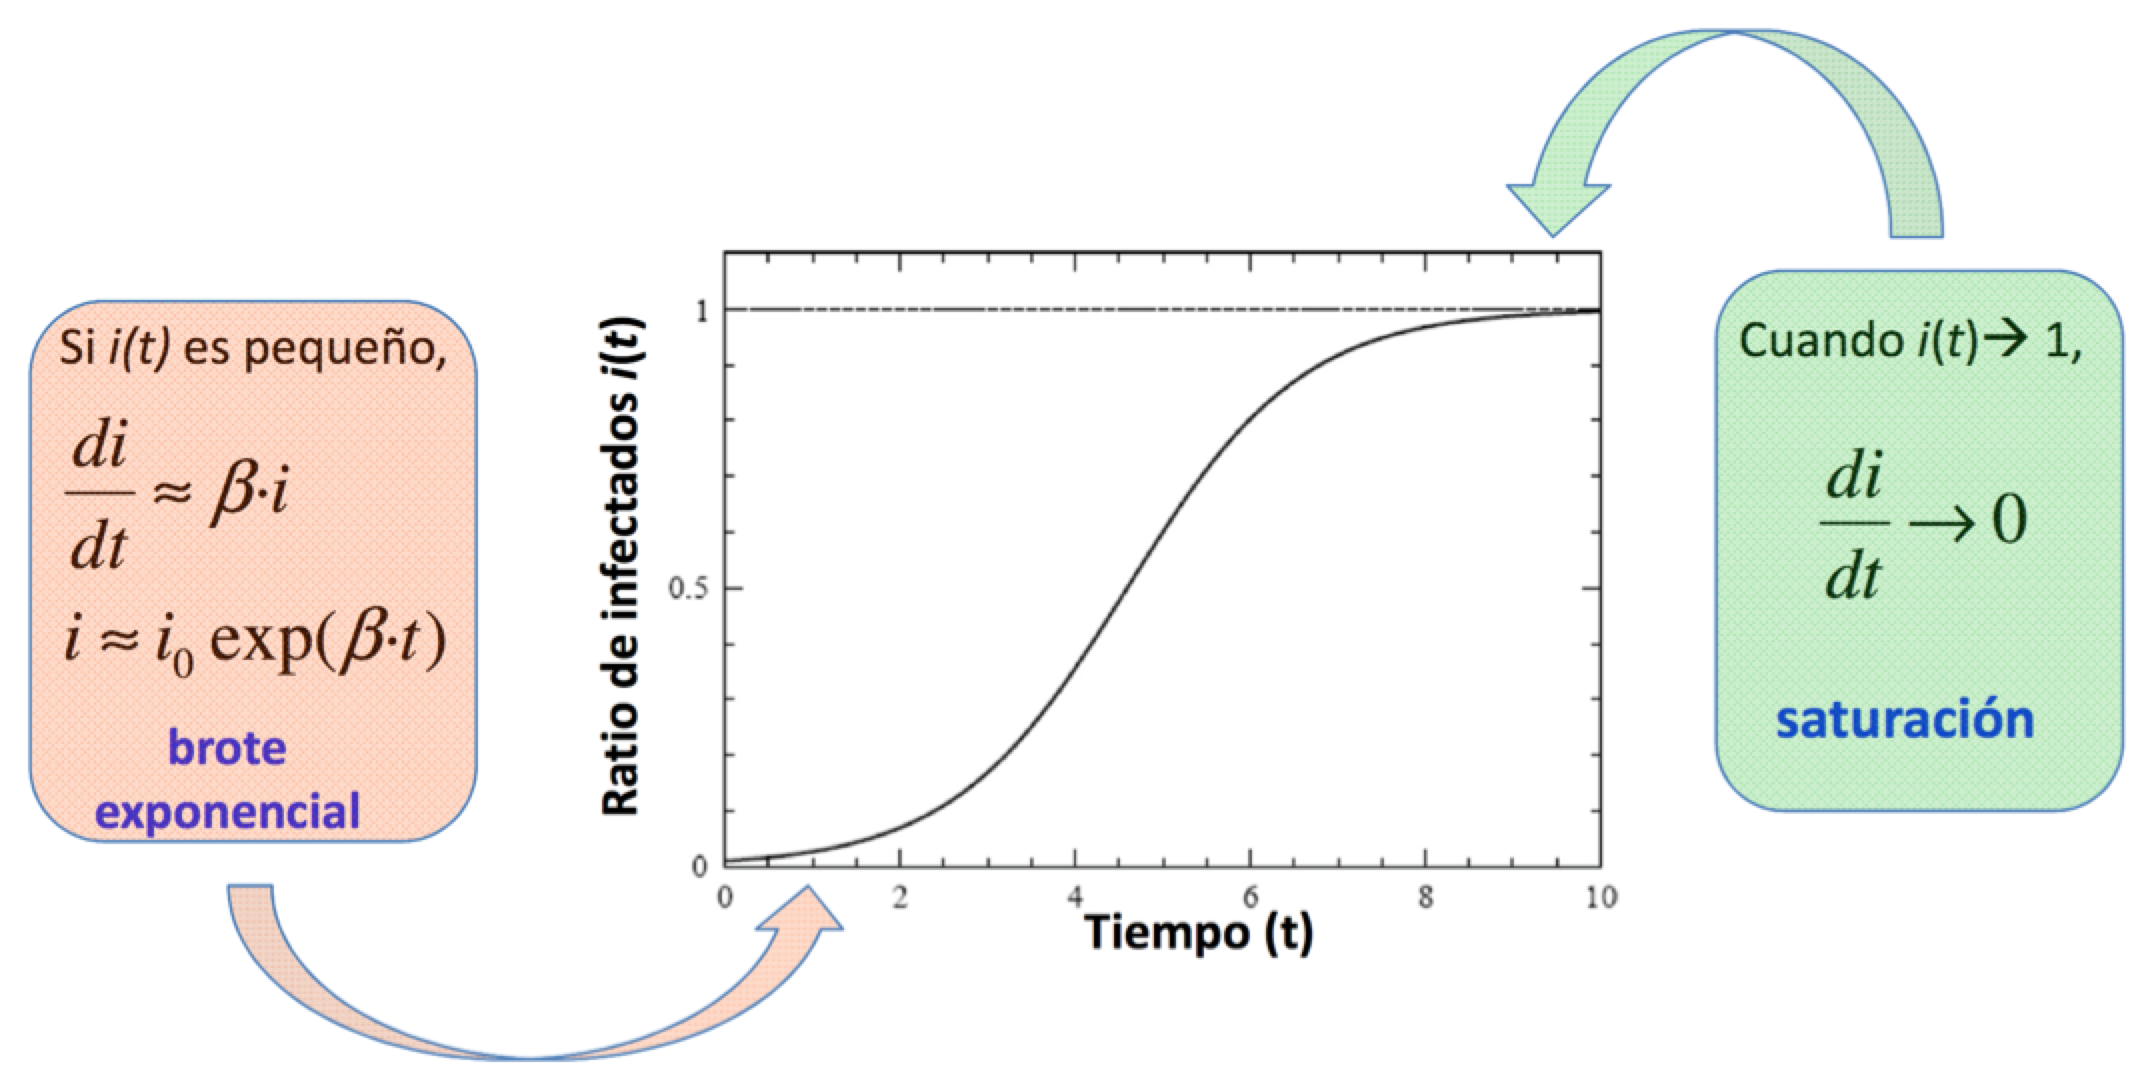
\includegraphics{../images/tema08/graficaSI.png}
\caption{Representación de la proporción de infectados en el Modelo SI}
\end{figure}

\subsubsection{Modelo SIS}\label{modelo-sis}

Es similar al anterior salvo en que, en este modelo, los individuos
infectados se pueden recuperar, volviendo al estado susceptible. Un
ejemplo de este modelo es el resfriado común.

\begin{figure}[htbp]
\centering
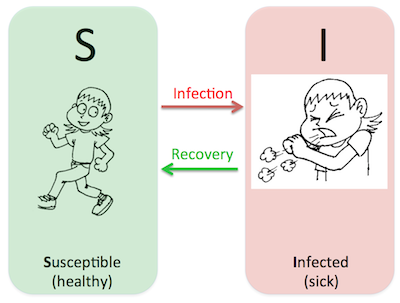
\includegraphics{../images/tema08/modeloSIS.png}
\caption{Esquema del Modelo SIS}
\end{figure}

Para este modelo necesitamos, además de los parámetros del anterior, la
tasa de recuperación \(\mu\), que representa la proporción de infectados
que se recuperan y pasan al estado susceptible en cada instante de
tiempo.

En este caso, la ecuación diferencial que modela la tasa a la que varía
el número de infectados es:

\[\frac{di}{dt} = i \cdot \beta  \cdot s - \mu \cdot i=  i \cdot \beta \cdot (1-i) - \mu \cdot i\]

En cada momento de tiempo, la proporción de infectados es la cantidad de
infectados \(i\) más la proporción de individuos susceptibles que pueden
ser infectados \(\beta \cdot s\) menos la proporción de individuos
infectados que se pueden recuperar \(\mu \cdot i\).

La resolución de esta ecuación nos da el siguiente resultado:

\[i = \Big(1- \frac{\mu}{\beta}\Big) \frac{C \cdot e^{(\beta - \mu)t}}{1 + C \cdot e ^{(\beta -\mu)t}}\]

\[C= \frac{\beta \cdot i_0}{\beta - \mu - \beta \cdot i_0}\]

En este caso, las conclusiones que podemos extraer de la representación
gráfica de la función son las siguientes:

\begin{itemize}
\itemsep1pt\parskip0pt\parsep0pt
\item
  Como la recuperación es posible, el sistema alcanza un \emph{estado
  endémico} en el que la tasa de infectados es constante:
\end{itemize}

\[i(\infty) = 1 - \frac{\beta}{\mu}\]

En este estado endémico, la proporción de infectados no varía con el
tiempo y sólo se produce cuando la tasa de recuperación es inferior a la
tasa de transmisión (\(\mu < \beta\))

\begin{figure}[htbp]
\centering
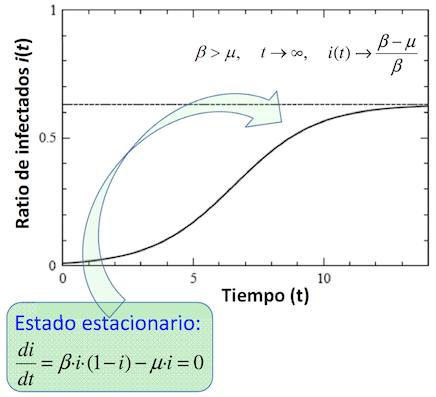
\includegraphics{../images/tema08/graficaSIS.png}
\caption{Representación de la proporción de infectados en el Modelo SIS}
\end{figure}

\begin{itemize}
\itemsep1pt\parskip0pt\parsep0pt
\item
  En caso de que la tasa de recuperación sea mayor que la tasa de
  transmisión (\(\mu > \beta\)) entonces llegado a un determinado punto
  la proporción de infectados comienza a decrecer exponencialmente,
  alcanzado un estado libre de enfermedad, en la que todos los
  individuos se han recuperado y no hay infectados.
\end{itemize}

El ritmo reproductivo básico (\(R_0\)) representa el número promedio de
individuos susceptibles que serán infectados por un individuo infectado:

\[R_0 = \frac{\beta}{\mu}\]

Tal y como hemos visto antes, si \(R_0<1\) entonces la enfermedad
termina desapareciendo de la población. Si \(R_0>0\) entonces la
enfermedad se propagará. Cuanto mayor sea \(R_0\), más rápido es el
proceso de propagación de la enfermedad. Por ejemplo, el sarampión (que
se contagia por el aire) tiene un \(R_0= 12-18\) mientras que la gripe
tiene un \(R_0 = 2-3\).

\subsubsection{Modelo SIR}\label{modelo-sir}

En este modelo, los individuos infectados no vuelven a ser susceptibles
sino que desarrollan una inmunidad a la enfermedad (o mueren) y pasan a
un estado recuperado\footnote{En inglés, el estado es \emph{removed},
  que es más adecuado para describir el proceso.} en el que no afectan
al modelo de propagación: no pueden ser infectados ni pueden infectar a
otros.

\begin{figure}[htbp]
\centering
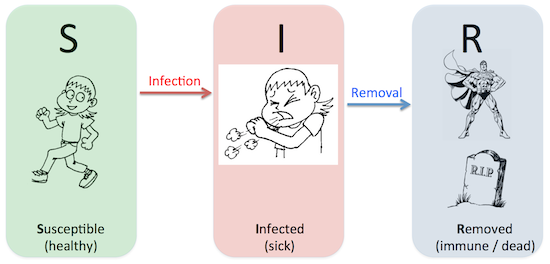
\includegraphics{../images/tema08/modeloSIR.png}
\caption{Esquema del Modelo SIR}
\end{figure}

En este modelo \(\mu\) representa la tasa de recuperación que, a
diferencia del anterior, es la tasa de individuos infectados que pasan
al estado recuperado. Para este modelo, la población es la suma de los
infectados, susceptibles y recuperados(\(R(t)\)), por lo que la
proporción de infectados es \(i = 1-s-r\).

Las ecuaciones diferenciales de este modelo son las siguientes:

\[\frac{di}{dt} = \beta \cdot i \cdot s - \mu \cdot i \text{;  }\frac{ds}{dt} = -\beta \cdot i \cdot s\text{;  }\frac{dr}{dt} = \mu \cdot i\]

En este caso el cálculo es más complejo pero podemos llegar a la
siguiente representación gráfica de las tres funciones:

\begin{figure}[htbp]
\centering
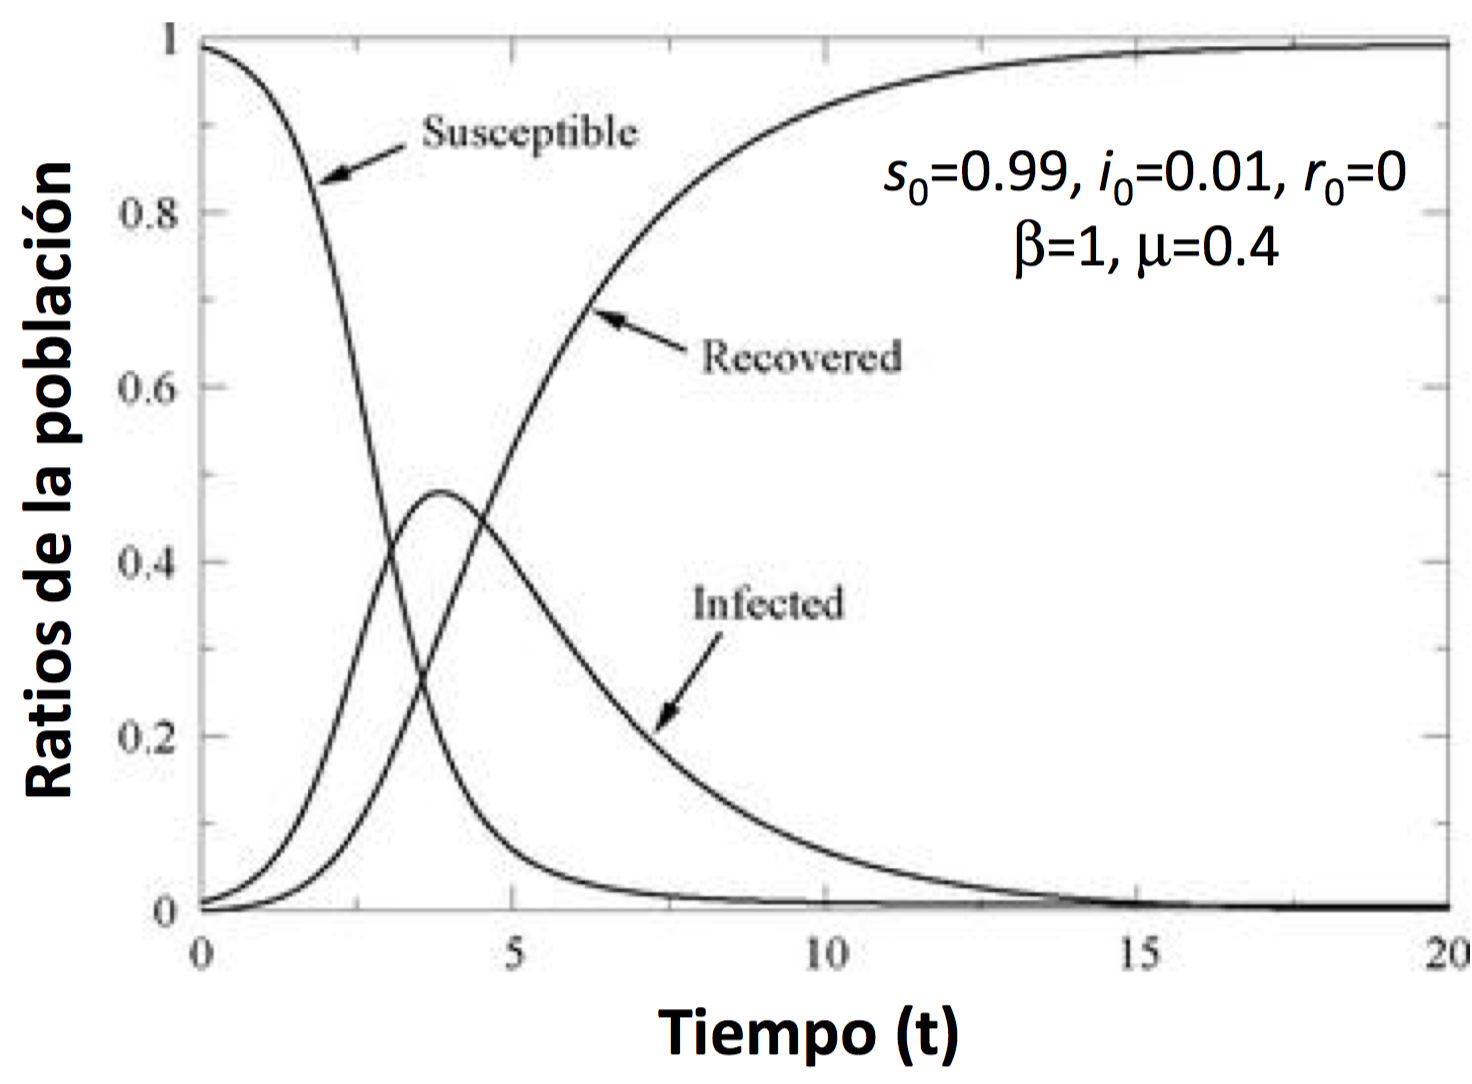
\includegraphics{../images/tema08/graficaSIR.png}
\caption{Representación de la proporción de infectados, susceptibles y
recuperados en el Modelo SIR}
\end{figure}

\begin{itemize}
\itemsep1pt\parskip0pt\parsep0pt
\item
  Cuando \(\beta>\mu\) la proporción de infectados crece hasta un pico
  máximo y luego decrece hasta valer 0.
\item
  La proporción de susceptibles decrece de forma monótona. Aunque
  satura, no llega nunca a 0 ya que cuando \(i \to 0\) ya no hay
  individuos que puedan infectar. Esto implica que los individuos que se
  mantienen susceptibles hasta fases avanzadas pueden no llegar a
  infectarse nunca.
\item
  La proporción de recuperados crece de manera monótona. De manera
  similar a los susceptibles, la proporción de recuperados nunca llega a
  valer 1. Su valor asintótico representa el número de individuos
  afectados y se calcula como:
\end{itemize}

\[r = 1- s_0 \cdot e^{-\beta \frac{r}{\mu}}\]

Las condiciones iniciales más habituales son:

\[i_0 = \frac{c}{N}\text{;  }s_0 = 1- \frac{c}{N}\text{;  }r_0 = 0\]

\subsubsection{Comportamientos importantes de los modelos
epidemiológicos}\label{comportamientos-importantes-de-los-modelos-epidemioluxf3gicos}

Existen principalmente dos comportamientos destacables en estos modelos:

\paragraph*{Comportamiento temprano.}\label{comportamiento-temprano.}
\addcontentsline{toc}{paragraph}{Comportamiento temprano.}

Es el patrón de comportamiento en las fases iniciales. Es importante
para saber cuánto tiempo tenemos para el desarrollo de vacunas e
intervenciones médicas. La mejor forma de detener o contener la epidemia
en esta fase es mediante vacunación temprana o la cuarentena.

En todos los modelos el número de infectados en la fase temprana es bajo
pero crece exponencialmente. Generalmente, el modelo SI es el más
relevante para describir este comportamiento.

\paragraph*{Comportamiento tardío.}\label{comportamiento-tarduxedo.}
\addcontentsline{toc}{paragraph}{Comportamiento tardío.}

Es el patrón de comportamiento en las fases más avanzadas de la epidemia
(cuando \(t \to \infty\)). Permite predecir el alcance, número de
infectados, etc.

En este caso, cada modelo realiza una predicción distinta:

\begin{itemize}
\itemsep1pt\parskip0pt\parsep0pt
\item
  En el modelo SI todos terminan infectados.
\item
  En el modelo SIS se alcanza un estado endémico en el que una
  proporción de la población queda infectada (\(R_0>1\)) o en el que la
  enfermedad desaparece (\(R_0<1\))
\item
  En el modelo SIR todos terminan recuperados (en el estado susceptible
  o recuperado, pero no infectados)
\end{itemize}

En resumen, las características básicas de los modelos epidemiológicos
son los siguientes:

\begin{figure}[htbp]
\centering
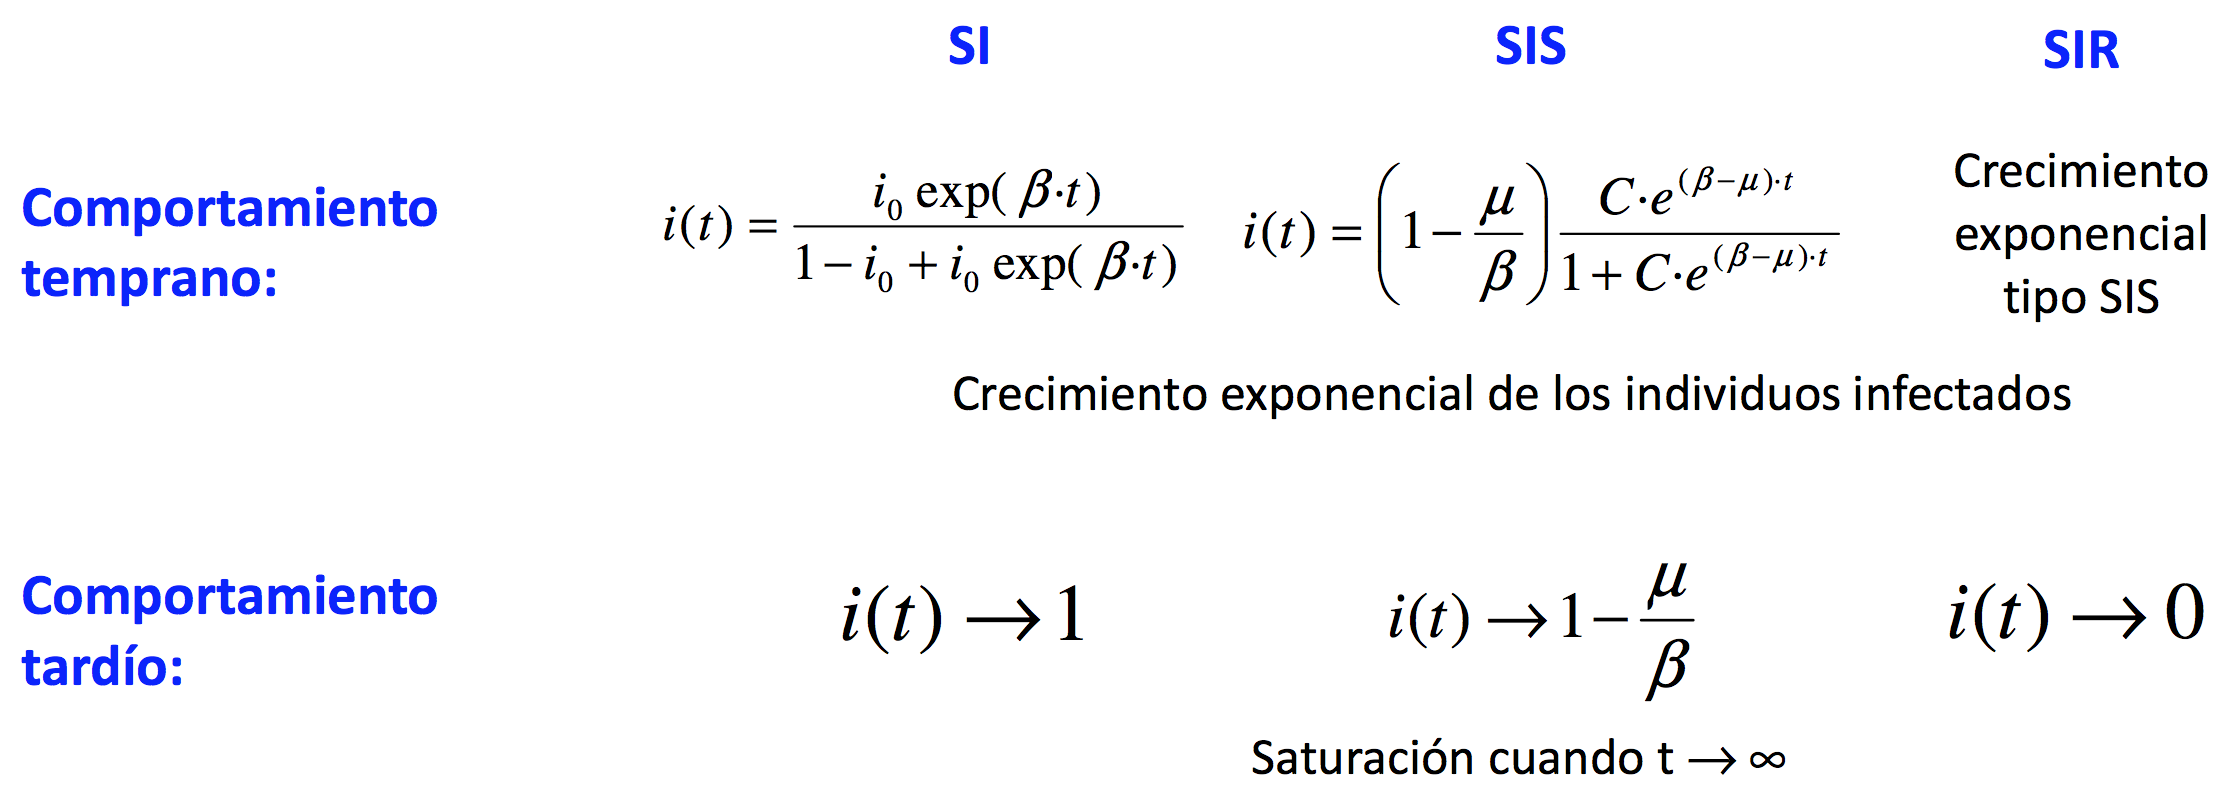
\includegraphics{../images/tema08/resumenModelos.png}
\caption{Características básicas de los modelos epidemiológicos}
\end{figure}

Tal y como hemos indicado, estos modelos no tienen en cuenta la red de
contactos ya que suponen que hay una mezcla homogénea. Realmente, las
epidemias se propagan a través de los contactos de las personas, es
decir, a través de los enlaces de su red social. Por tanto, hay que
tener en cuenta el papel de la red en el proceso epidémico. Tal y como
veremos a continuación, la estructura de la red modificará el
comportamiento de estos modelos simples.

\subsection{Modelos de contagio basados en
redes}\label{modelos-de-contagio-basados-en-redes}

Los modelos de contagio basados en redes se comportan de manera similar
a los vistos hasta ahora salvo que solo se tendrán en cuenta los
contactos definidos por la red, en lugar de suponer que cualquier
individuo puede estar en contacto con cualquier otro.

En los modelos basados en redes, \(\beta\) es el \textbf{ratio de
transmisión} y representará la probabilidad de contagio de un nodo
infectado a otro susceptible que esté en contacto con él (hay un enlace
entre los dos nodos).

En general, la simulación de estos procesos suele ser más sencilla que
la resolución analítica de los modelos en redes complejas. Por ejemplo,
una forma sencilla de simular un proceso de contagio simple sería la
siguiente:

\begin{enumerate}
\def\labelenumi{\arabic{enumi}.}
\itemsep1pt\parskip0pt\parsep0pt
\item
  Definimos una red de \(N\) nodos y \(L\) enlaces. Inicialmente todos
  los nodos están en el estado S.
\item
  En \(t_0\) ponemos una pequeña fracción \(i_0\) de nodos (o solo 1),
  en el estado I.
\item
  En cada paso de tiempo, hacemos que cada uno de los nodos en el estado
  I\footnote{Desde el punto de vista de implementación, es recomendable
    tener en listas separadas los nodos infectados y los susceptibles (y
    recuperados) no tener que procesar todos los nodos (solo los
    infectados) y así optimizar el proceso de simulación.} propague la
  infección a cada uno de sus vecinos en estado S con probabilidad
  \(\beta\) (al igual que en los modelos de red aleatoria o
  Barabasi-Albert, generamos un número aleatorio \(a\) y propagamos si
  \(a<\beta\)).
\item
  En caso de utilizar un modelo SIR o SIS, haremos que los nodos en
  estado I puedan pasar al estado R (o S, dependiendo del modelo), con
  una probabilidad \(\mu\).
\end{enumerate}

Existen alternativas más complejas (y más realistas), basadas en
técnicas de modelado social o modelado basado en agentes, en los que
cada individuo (nodo) se modela como un agente que puede incluir sus
propias características individuales y que pueden generar
comportamientos emergentes. Se pueden incluir procesos estocásticos de
actualización de estados que simulan eventos aleatorios que pueden
ocurrir en los procesos dinámicos.

Dependiendo del fenómeno de difusión que queramos simular tendremos que
decidir qué red tendremos que modelar. Como ejemplo podemos ver que
redes se usan para modelar distintos fenómenos en la siguiente tabla:

\begin{figure}[htbp]
\centering
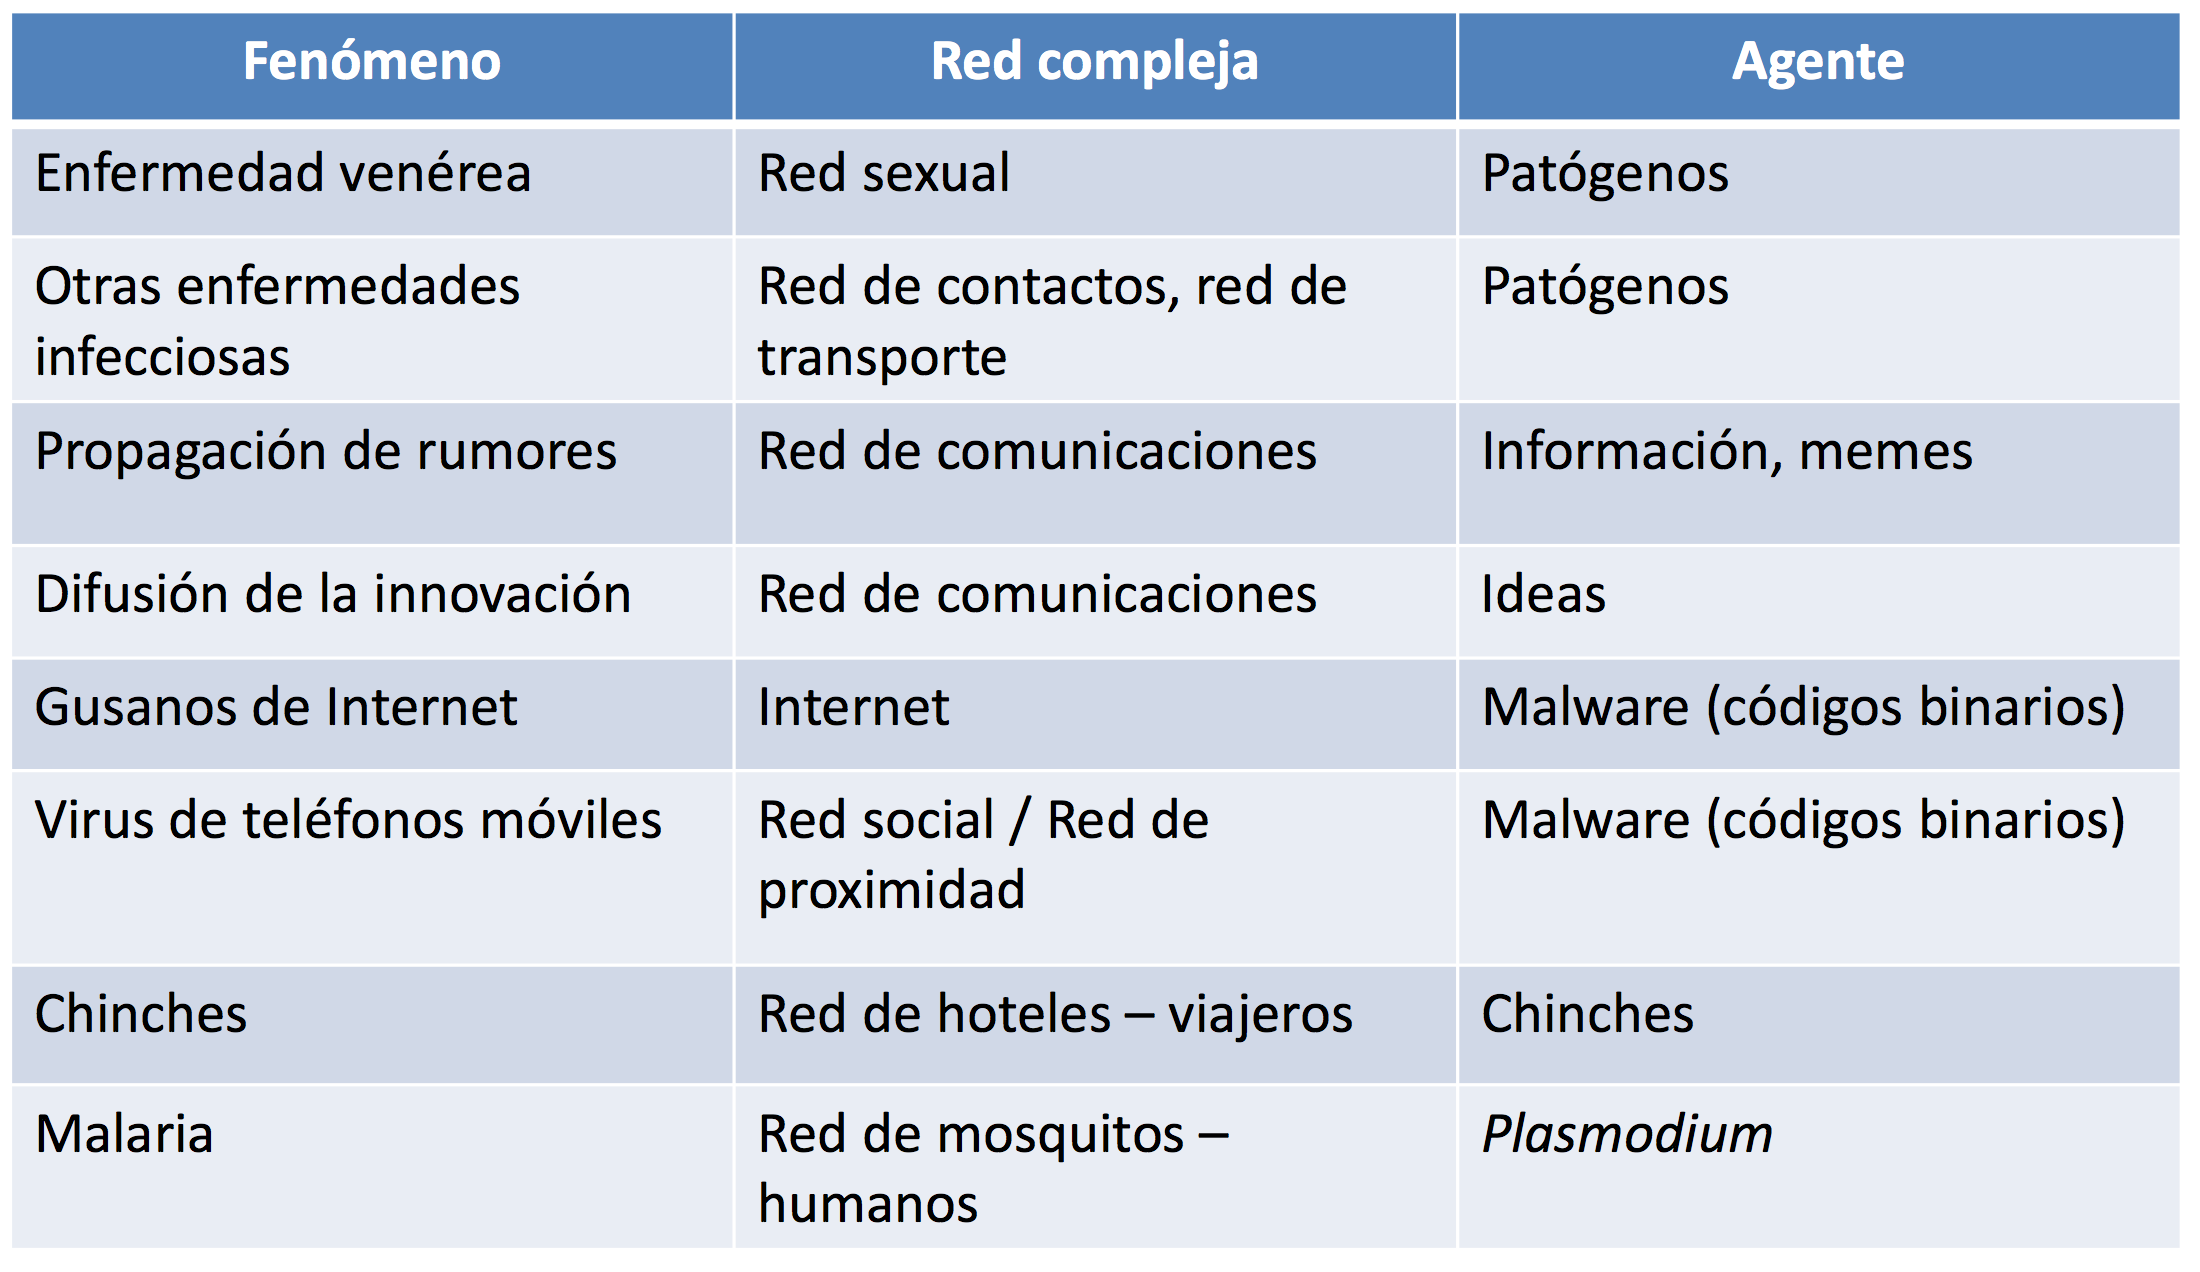
\includegraphics{../images/tema08/tabla.png}
\caption{Modelados de fenómenos de contagio y redes utilizadas}
\end{figure}

La estructura de la red, su evolución a lo largo del tiempo y su uso
están interrelacionados y se deben estudiar conjuntamente. La topología
de la red va a influir en el proceso de contagio o difusión:

\begin{itemize}
\itemsep1pt\parskip0pt\parsep0pt
\item
  ¿A qué estado convergen los nodos?
\item
  ¿Cuánto se tarda en llegar a dicho estado?
\item
  ¿Cómo se puede inmunizar un sistema complejo con una topología de red
  concreta?
\end{itemize}

Antes de entrar en los detalles más analíticos de los procesos de
difusión vamos a utilizar los modelos que conocemos hasta ahora y las
simulaciones en NetLogo para observar el comportamiento de las epidemias
teniendo en cuenta la estructura de la red.

\subsubsection{Redes aleatorias}\label{redes-aleatorias}

Vamos a simular un modelo SI en una red aleatoria. Si utilizamos el
simulador de
\href{http://www.ladamic.com/netlearn/NetLogo501/ERDiffusion.html}{Difusión
en una red aleatoria}\footnote{Todos los modelos de NetLogo que se ven
  en este tema están disponibles en el Campus Virtual.} podemos ver la
influencia de la densidad de la red en los procesos de contagio.

\begin{figure}[htbp]
\centering
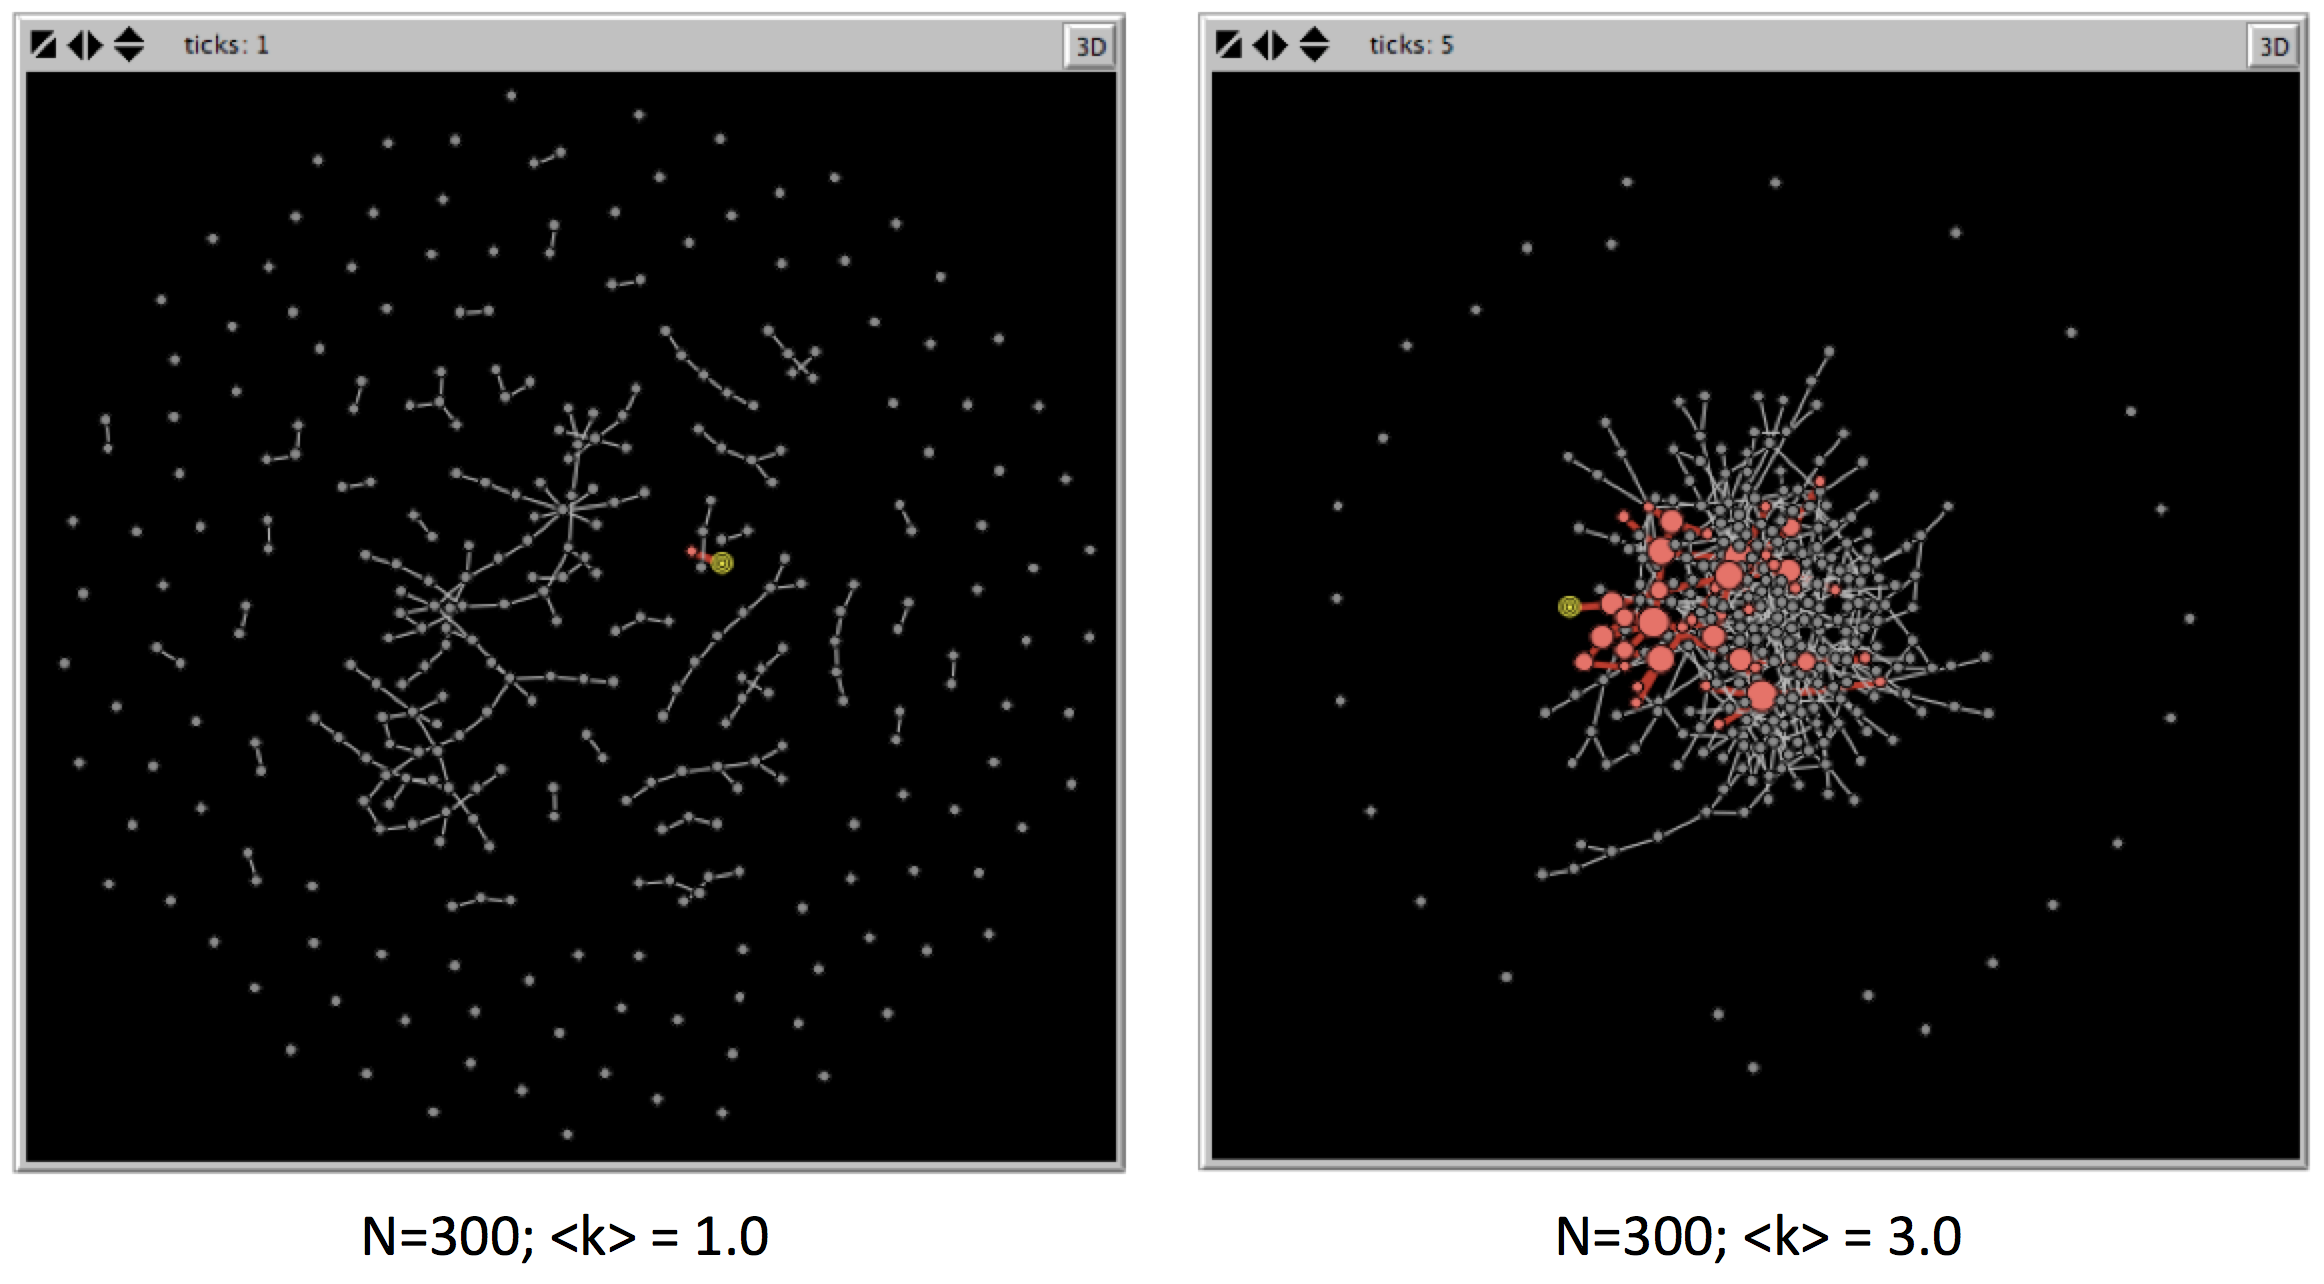
\includegraphics{../images/tema08/contagioER.png}
\caption{Influencia de la densidad de la red aleatoria en los procesos
de contagio}
\end{figure}

Como se puede ver en la simulación, la densidad de la red afecta a la
velocidad de infección y al número de individuos infectados: a mayor
densidad, mayor es el número de individuos infectados y mayor es la
velocidad de propagación.

Además, se puede ver que si partimos de un único nodo, sólo se
infectarán los nodos que pertenecen a la misma componente conexa.
Recordemos algunas redes reales tienen una componente gigante y muchas
componentes pequeñas por lo que la epidemia se extiende en mayor o menor
medida dependiendo de la localización del nodo inicial. La probabilidad
de que un nodo pertenezca a la componente gigante se \(\frac{N_G}{N}\).

\subsubsection{Redes libres de escala}\label{redes-libres-de-escala}

A continuación simularemos un modelo SI en una red libre de escala
creada siguiendo el modelo de Barabasi-Albert. Si recordamos, para que
se presente la propiedad de ser libre de escala es necesario que exista
enlace preferencial. Por este motivo vamos a ver el efecto de la
existencia de enlace preferencial en estas redes. Para ello usaremos el
simulador de
\href{http://www.ladamic.com/netlearn/NetLogo501/BADiffusion.html}{Difusión
en una red libre de escala}.

\begin{figure}[htbp]
\centering
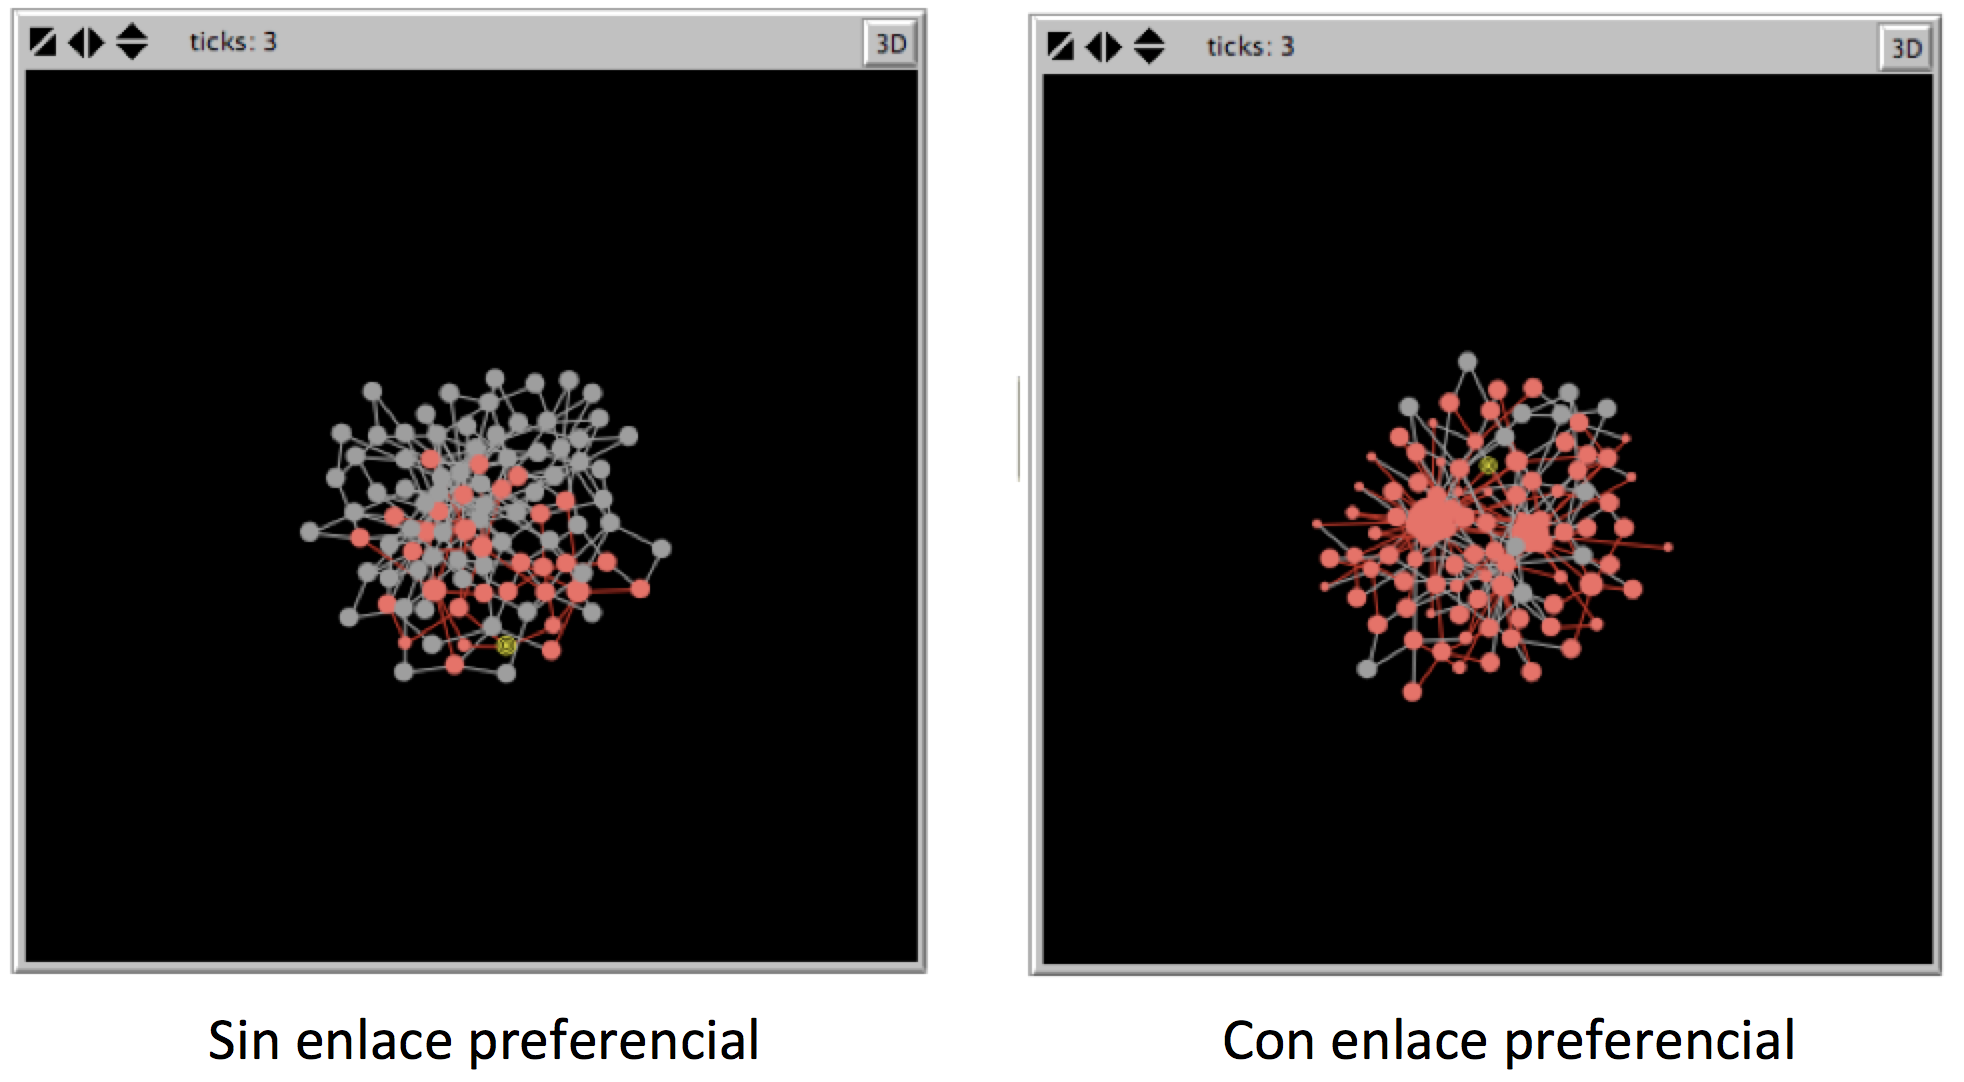
\includegraphics{../images/tema08/contagioBA.png}
\caption{Influencia del enlace preferencial (redes libres de escala) en
los procesos de contagio}
\end{figure}

En este caso podemos observar que el enlace preferencial favorece el
contagio. Esto se debe a que el enlace preferencial posibilita la
existencia de Hubs, que son los responsables de ayudar a difundir más
rápidamente la infección.

\subsubsection{Redes de Watts-Strogatz}\label{redes-de-watts-strogatz}

En este caso simularemos un modelo SI en una red creada siguiendo el
modelo de Watts-Strogatz para estudiar la influencia de los ``atajos'' o
enlaces débiles en el contagio sobre esta red. Para ello vamos a usar el
simulador
\href{http://www.ladamic.com/netlearn/NetLogo4/SmallWorldDiffusionSIS.html}{Difusión
en un mundo pequeño} y modificaremos la probabilidad de reasignación de
enlaces \(p\) para ver su efecto en la propagación.

\begin{figure}[htbp]
\centering
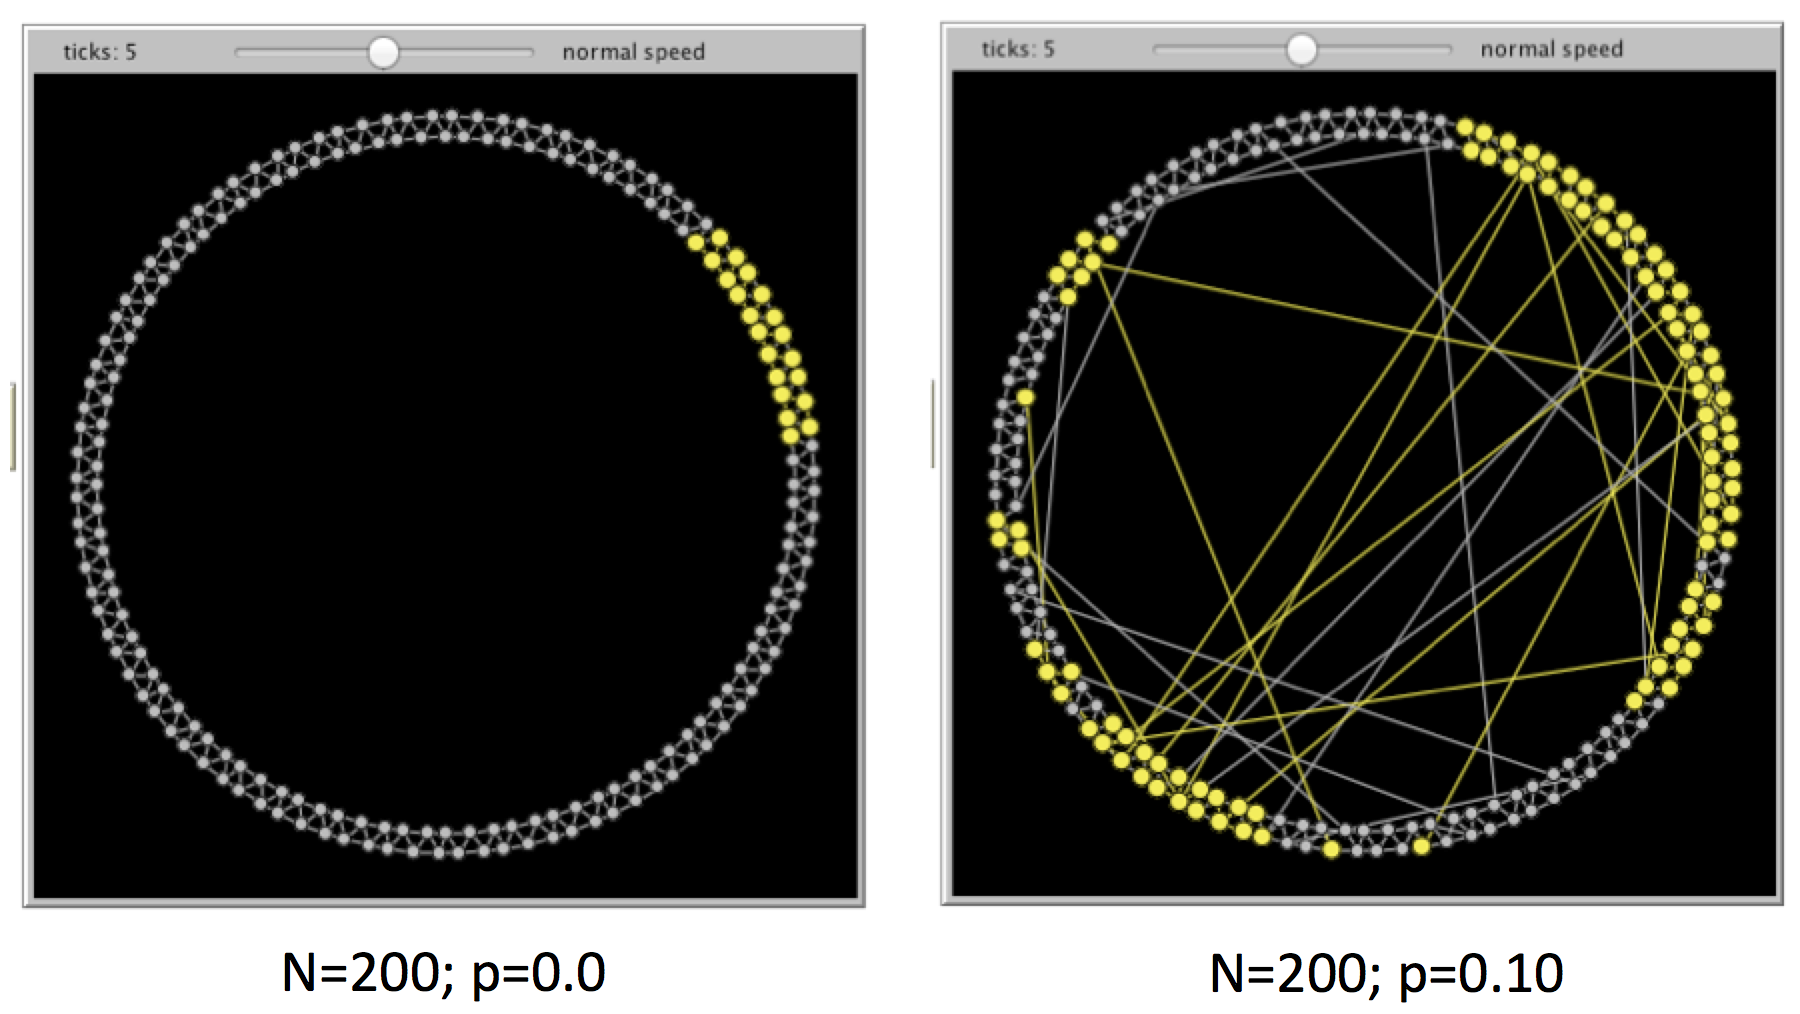
\includegraphics{../images/tema08/contagioSW.png}
\caption{Influencia de los enlaces débiles en los procesos de contagio}
\end{figure}

Podemos observar que los enlaces débiles provocan que aumente la
velocidad de la infección ya que, en el mismo tiempo, se aprecia un
mayor número de nodos infectados.

\subsubsection{Soluciones analíticas}\label{soluciones-analuxedticas}

Podemos estudiar de manera analítica el comportamiento temprano y tardío
de los modelos de contagio SI y SIR en redes complejas. Para ello es
necesario hacer una aproximación conocida como la \textbf{aproximación
por bloques de grados}: distinguimos distintos bloques de nodos basados
en el grado que tienen y asumimos que todos los nodos en el mismo bloque
(y, por tanto, con el mismo grado) son estadísticamente equivalentes.
Podemos representarlo gráficamente con la siguiente figura:

\begin{figure}[htbp]
\centering
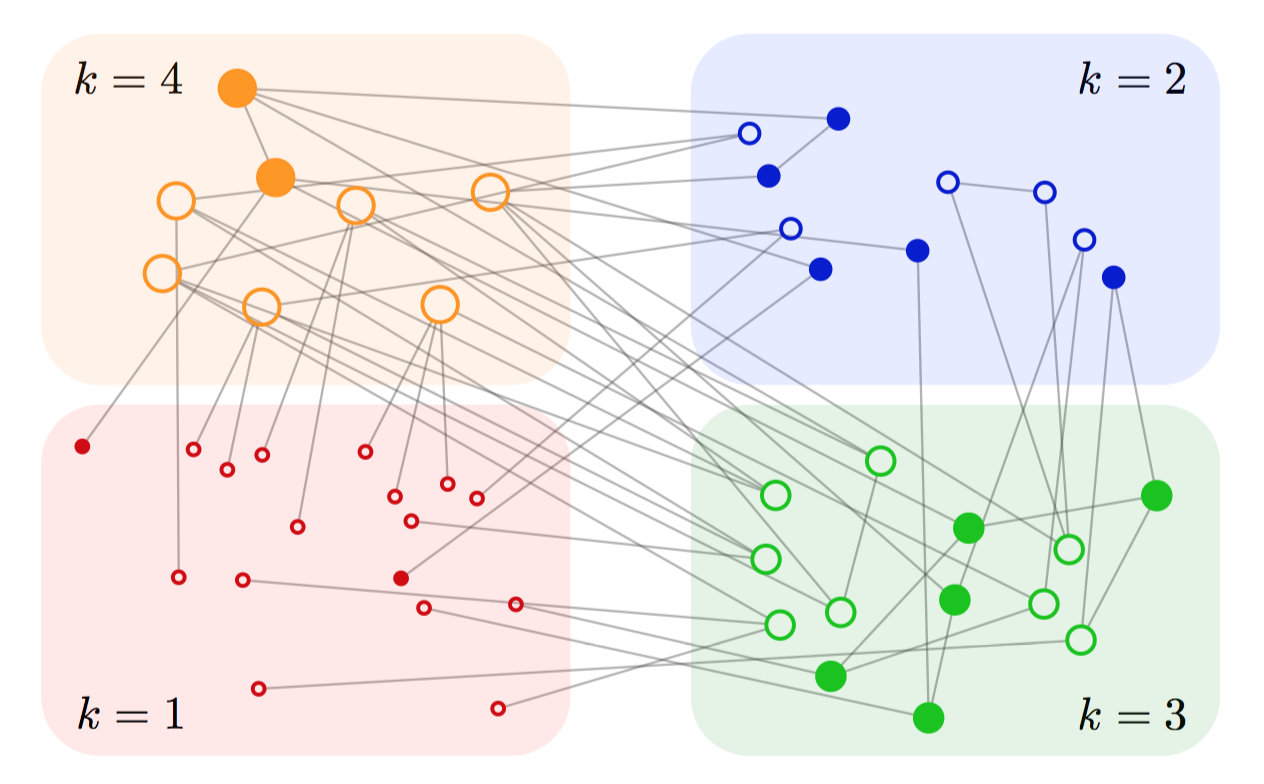
\includegraphics{../images/tema08/bloqueGrado.png}
\caption{Aproximación por bloques de grados}
\end{figure}

De esta forma definimos la fracción de nodos con grado \(k\) infectados
como:

\[i_k  = \frac{I_k}{N_k}\]

La suma de los diferentes \(i_k\) para todos los grados dan la fracción
total de nodos infectados \(i\).

\paragraph*{Modelo SI}\label{modelo-si-1}
\addcontentsline{toc}{paragraph}{Modelo SI}

De acuerdo a lo anterior, definimos la ecuación diferencial para el
modelo SI que modela la tasa de infectados para cada grado \(k\) por
separado:

\[\frac{di_k}{dt} = \beta (1-i_k(t))k \Theta_k(t)\]

En este caso:

\begin{itemize}
\itemsep1pt\parskip0pt\parsep0pt
\item
  El grado medio ha sido sustituido por el grado real \(k\)
\item
  \(\Theta_k(t)\) es una función de densidad que representa la fracción
  de vecinos que están infectados para un nodo de grado \(k\).
\item
  Necesitaremos definir \(k_{max}\) ecuaciones.
\end{itemize}

La función de densidad podemos aproximarla de la siguiente forma:

\[\Theta_k(t) \approx \Theta(t) = \frac{\sum_{k'}(k'-1)\cdot P(k') \cdot i_{k'}(t)}{\langle k \rangle}\]

Durante el comportamiento temprano, es decir, cuando \(i\) es pequeño
podemos aproximarlo de la siguiente forma:

\[\frac{di_k}{dt} = \beta k i_0 \frac{\langle k \rangle-1}{\langle k \rangle} e^{t/\tau}\]

Y podemos obtener la fracción de nodos infectados de grado \(k\) y el
total de nodos infectados:

\[i_k = i_0 (1+ \frac{k \langle k \rangle -1}{\langle k^2 \rangle - \langle k \rangle}(e^{t/\tau}-1))\]

\[i = i_0 (1+ \frac{\langle k \rangle^2 - \langle k \rangle}{\langle k^2 \rangle - \langle k \rangle}(e^{t/\tau}-1))\]

\(\tau\) representa el periodo de incubación, que es la cantidad de
tiempo que requiere la epidemia para crecer. Cuando menor es \(\tau\),
más rápido se propaga la enfermedad. Según las ecuaciones anteriores se
puede calcular de la siguiente forma:

\[\tau = \frac{\langle k \rangle}{\beta(\langle k^2 \rangle - \langle k \rangle)}\]

De estas ecuaciones podemos obtener las siguientes conclusiones:

\begin{itemize}
\itemsep1pt\parskip0pt\parsep0pt
\item
  Cuanto mayor sea el grado de un nodo mayor es la probabilidad de que
  ese nodo sea infectado.
\item
  El periodo de incubación depende de la estructura de la red y de los
  momentos de primer y segundo orden de la distribución de grados
  (\(\langle k \rangle\) y \(\langle k^2 \rangle\)), respectivamente.
\item
  En una red aleatoria el periodo de incubación depende de la densidad
  de la red, de modo que la epidemia se propaga más rápido cuanto más
  densa sea ésta (mayor \(\langle k \rangle\)).
\end{itemize}

\[\tau_{ER} = \frac{1}{\beta(\langle k \rangle)} \text{ ya que } \langle k^2 \rangle = \langle k \rangle (\langle k \rangle - 1)\]

\begin{itemize}
\itemsep1pt\parskip0pt\parsep0pt
\item
  En una red libre de escala los momentos dependen de \(\gamma\), de
  modo que si \(\gamma \geq 3\) ambos momentos son finitos y el contagio
  se comporta de manera similar a la red aleatoria.
\item
  Sin embargo, si \(\gamma < 3\) en una red libre de escala entonces
  \(\langle k^2 \rangle\) diverge y \(\tau \to 0\), lo que implica que
  el periodo de incubación característico desaparece y la epidemia es
  instantánea. Esto se debe a que los hubs son los primeros nodos en
  infectarse y, dada su alta conectividad, infectan más rápidamente a la
  mayoría de los nodos.
\end{itemize}

\paragraph*{Modelos SIS}\label{modelos-sis}
\addcontentsline{toc}{paragraph}{Modelos SIS}

En los modelos con recuperación la ecuación diferencial de la tasa de
infectados de grado \(k\) es algo distinta:

\[\frac{di_k}{dt} = \beta (1-i_k(t))k \Theta_k(t) _ \mu \cdot i_k(t)\]

Donde vemos que aparece la tasa de recuperación \(\mu\). Esto hace que
el periodo de incubación \(\tau\) sea algo distinto:

\[\tau^{SIS} = \frac{\langle k \rangle}{\beta \langle k^2 \rangle - \mu \langle k \rangle}\]

Para un tamaño suficientemente grande de \(\mu\) el tiempo
característico se hace negativo e \(i_k\) decrece exponencialmente. Sin
embargo, depende de la topología de la red. En lugar de solo \(\mu\)
vamos a tener en cuenta el ritmo reproductivo básico
\(\lambda = \frac{\beta}{\mu}\), que es representativo de la enfermedad
(o de lo que queremos difundir) y que cuanto mayor sea más probable es
que la enfermedad se propague. Sin embargo, ¿cuál es el mínimo valor
necesario para que se propague la enfermedad? Esto es lo que se conoce
como el \textbf{umbral epidemiológico} (\(\lambda_C\))y también
dependerá de la estructura de la red.

\begin{itemize}
\itemsep1pt\parskip0pt\parsep0pt
\item
  Para una red aleatoria tenemos que el umbral epidemiológico es:
\end{itemize}

\[\lambda_C = \frac{1}{\langle k \rangle +1}\]

Esto implica que siempre va a ser distinto de cero y que, dependiendo
del valor de \(\lambda\), podemos conseguir que la epidemia alcance un
estado endémico (si \(\lambda > \lambda_C\)) o que la epidemia
desaparezca (si \(\lambda < \lambda_C\)).

\begin{itemize}
\itemsep1pt\parskip0pt\parsep0pt
\item
  Para una red libre de escala tenemos que el umbral epidemiológico es:
\end{itemize}

\[\lambda_C = \frac{\langle k \rangle}{\langle k^2 \rangle}\]

Esto implica que para \(\gamma < 3\) el segundo momento diverge y, por
tanto, el umbral epidemiológico desaparece. Esto implica que incluso las
enfermedades que son difíciles de transmitir se pueden propagar en una
red libre de escala. De nuevo, esto es consecuencia de los hubs: en el
momento en el que la enfermedad infecta un hub puede pasar a un número
muy grande de nodos, de modo que persiste en la población.

Para el modelo SIR los resultados son similares. En la siguiente tabla
se resumen las principales conclusiones extraídas:

\begin{figure}[htbp]
\centering
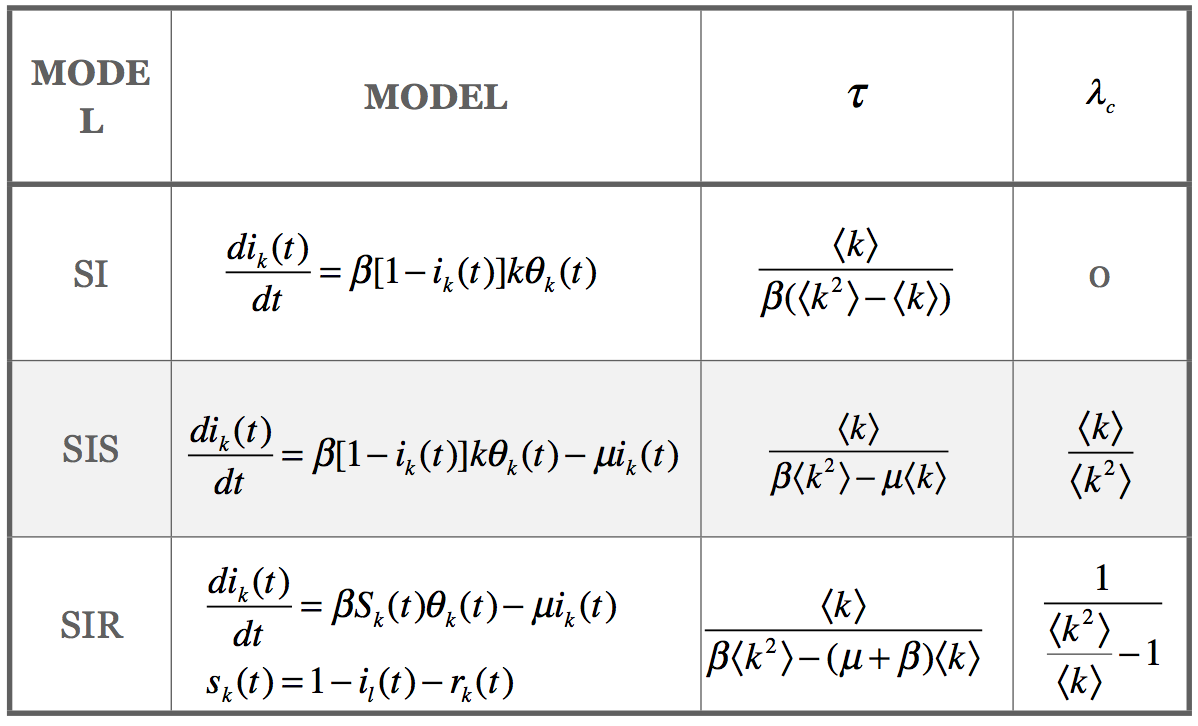
\includegraphics{../images/tema08/resumenModelosRedes.png}
\caption{Resumen de los modelos epidémicos en redes (Network Science,
cap. 10)}
\end{figure}

\subsection{Modelos de contagio
complejo}\label{modelos-de-contagio-complejo}

Hasta ahora hemos estudiado modelos de contagio simple, en los que el
contagio se produce uno a uno, es decir, basta con que un vecino de un
determinado nodo esté infectado para que se pueda quedar infectado. Sin
embargo, en algunos procesos como el contagio social o inducir a comprar
un producto, no basta con que uno de mis vecinos tenga una determinada
``opinión'' para cambiar la mía sino que es necesario sea una fracción
de mis vecinos. Esto es lo que se conoce como contagio complejo o
\textbf{contagio basado en umbrales}.

Existen principalmente dos formas de definir el contagio basado en
umbrales:

\begin{itemize}
\itemsep1pt\parskip0pt\parsep0pt
\item
  Mediante un umbral \(k\) que define el número de vecinos que han de
  estar infectados para que un nodo quede infectado. El modelo de
  contagio simple es un modelo basado en este tipo de umbral con
  \(k=1\).
\item
  Mediante una proporción \(p\) que define el porcentaje de vecinos que
  han de estar infectados para que un nodo quede infectado.
\end{itemize}

En este caso, la propagación se comporta de una manera bastante distinta
que depende principalmente de:

\begin{itemize}
\itemsep1pt\parskip0pt\parsep0pt
\item
  La estructura de la red.
\item
  El valor del umbral utilizado.
\item
  La elección de los nodos inicialmente infectados.
\end{itemize}

A modo de ejemplo podemos ver la diferencia entre un contagio simple y
uno complejo en un solo paso de simulación en la figura que aparece a
continuación. Como se puede ver, el contagio simple se propaga de una
manera mucho más rápida. Además, el contagio simple permite llegar a
toda la red (en la Figura, en \(t=2\) todos los nodos estarían
contagiados). Sin embargo, el contagio complejo es mucho más lento y
puede verse detenido rápidamente debido a la falta de conexiones (en la
Figura, en \(t=2\) solo J sería infectado y la infección se detendría).

\begin{figure}[htbp]
\centering
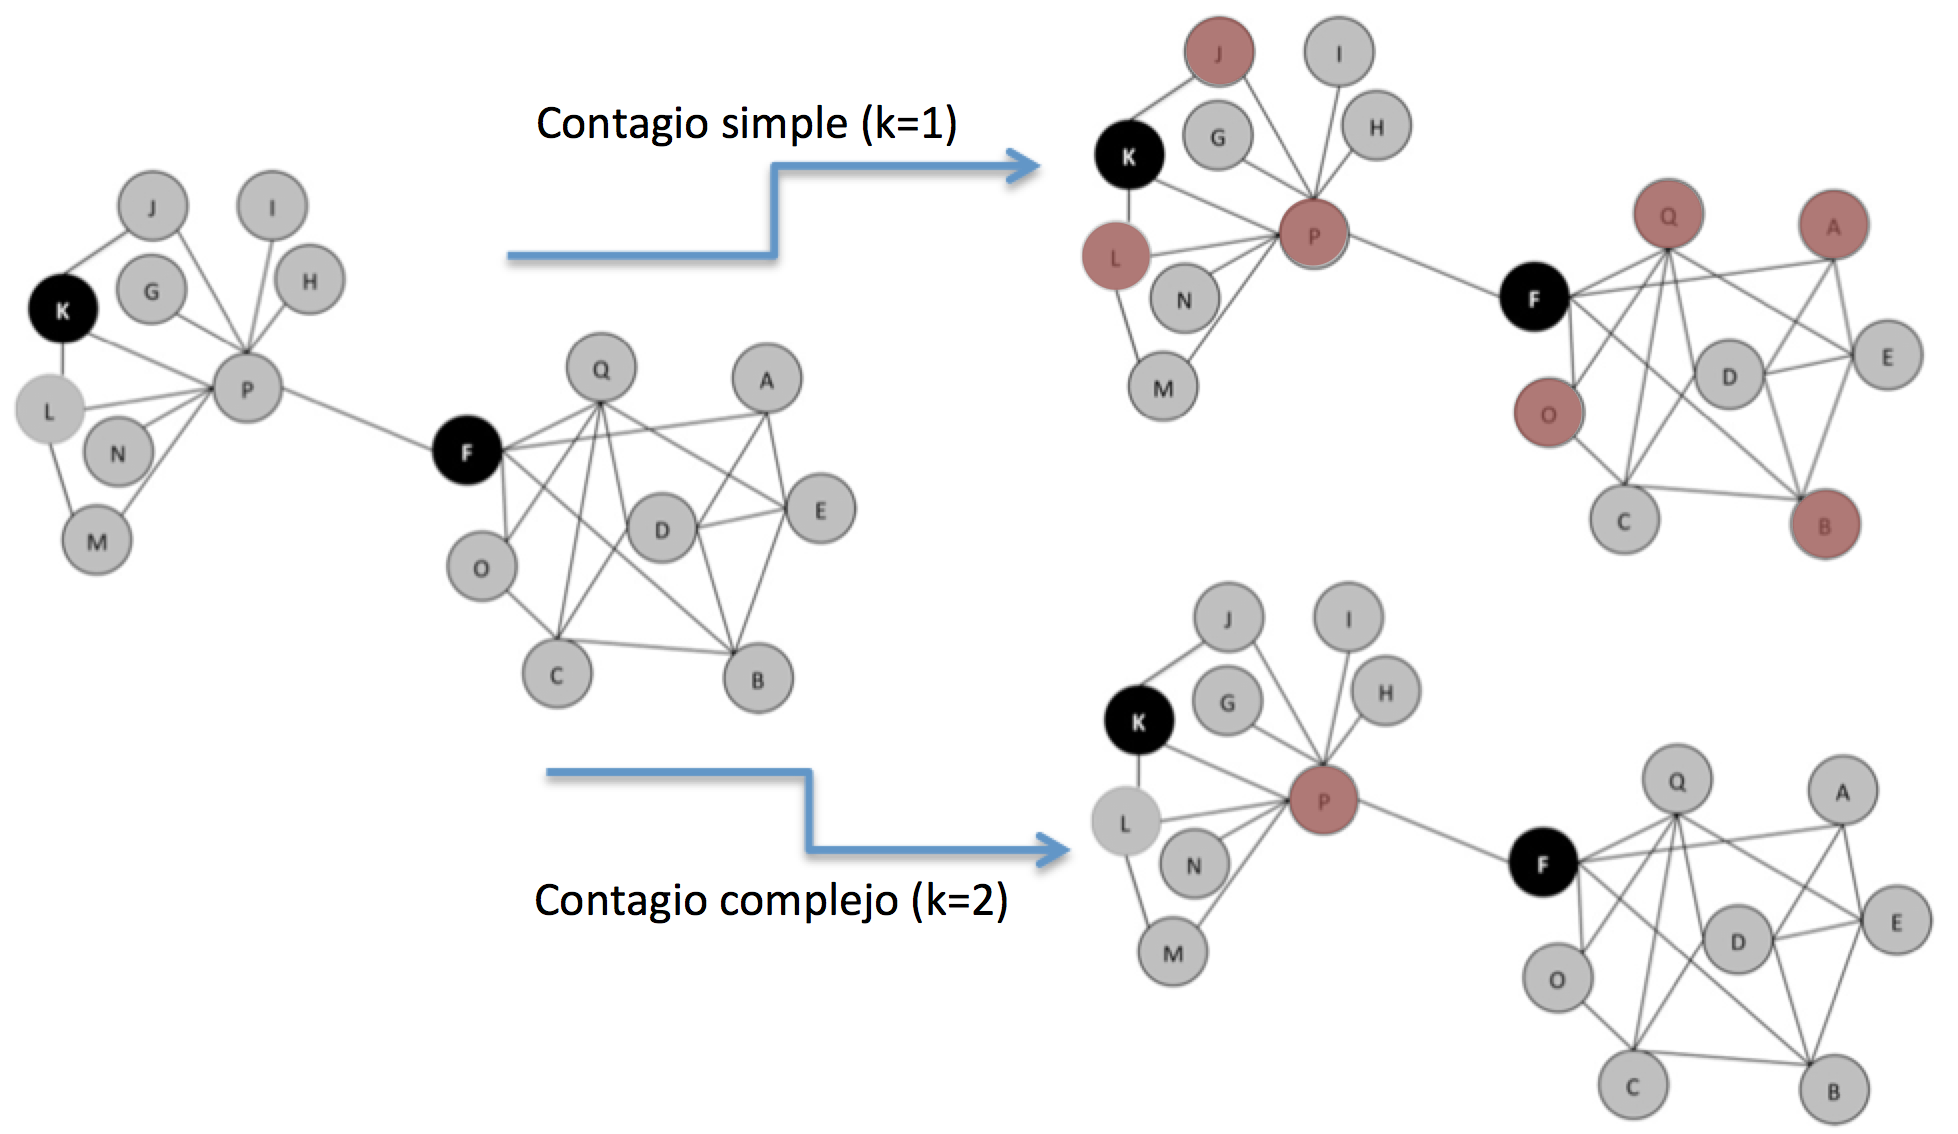
\includegraphics{../images/tema08/contagioComplejo.png}
\caption{Contagio simple vs.~Contagio complejo}
\end{figure}

Podemos ver también que los modelos de contagio complejos se comportan
de manera distinta en los modelos de redes vistos:

\begin{itemize}
\itemsep1pt\parskip0pt\parsep0pt
\item
  En una red de mundo pequeño (Watts-Strogatz) los enlaces débiles o
  atajos ya no funcionan como medio para aumentar la velocidad de
  propagación. Podemos ver este comportamiento en la simulación del
  modelo de contagio complejo en una red de mundo pequeño que hemos
  dejado en el Campus Virtual.
\item
  En una red libre de escala, los hubs pierden importancia en la
  velocidad de propagación ya que, aunque llegan a muchos nodos, solo
  ellos no son capaces de propagar la enfermedad.
\item
  En una red aleatoria la propagación depende muy decisivamente de los
  nodos inicialmente infectados.
\end{itemize}

\subsection{Modelos de difusión de opinión en
redes}\label{modelos-de-difusiuxf3n-de-opiniuxf3n-en-redes}

Aunque el modelo de contagio complejo basado en umbrales puede ser
adecuado para algunos procesos de difusión, existen otros modelos más
adecuados para modelar los procesos de difusión de opinión en redes.

Los modelos basados en \emph{efectos de beneficio directo} se basan en
que la adopción de una opinión se ve reforzada por el beneficio que se
consigue por la adopción de dicha opinión. Además, estos beneficios son
mayores cuantos más vecinos adopten esa misma opinión.

\subsubsection{Juego de coordinación en
redes}\label{juego-de-coordinaciuxf3n-en-redes}

Este modelo se puede simular mediante el \textbf{juego de coordinación
en una red}. En este modelo, cada nodo tiene que elegir entre dos
posibles opciones (que llamaremos A y B) y existe un beneficio si dos
nodos conectados eligen la misma opción. De una manera más formal
definimos el modelo de la siguiente forma:

\begin{itemize}
\itemsep1pt\parskip0pt\parsep0pt
\item
  Si dos nodos eligen la opción A entonces obtienen un beneficio de
  valor \(a>0\).
\item
  Si dos nodos eligen la opción B entonces obtienen un beneficio de
  valor \(b>0\)
\item
  \(p\) es la fracción de vecinos que adoptan la opción A, mientras que
  \((1-p)\) es la fracción de vecinos que adoptan la opción B.
\item
  Para un nodo de grado \(k\) podemos decir que este nodo adopta la
  opción A si:
\end{itemize}

\[p \cdot k \cdot a \geq (1-p) \cdot k \cdot b\]

Esto se puede convertir en un modelo de difusión basado en umbrales,
donde el umbral \(q\) tiene el valor:

\[q = \frac{b}{a+b}\]

Es decir, si tenemos una proporción de \(q\) vecinos que han adoptado la
opción A entonces elegiremos la opción A. En otro caso, nos es más
beneficioso adoptar la opción B.

El sistema tiene dos estados de equilibrio posibles: o todos adoptan la
opción A o, por el contrario, todos adoptan la opción B. Sin embargo, la
pregunta es qué pasaría si, partiendo de un estado de equilibrio,
algunos nodos (adoptadores iniciales) cambian su opción de manera
aleatoria. Queremos saber si se va a producir una propagación en cascada
de este comportamiento o si, por el contrario, este comportamiento se
detendrá en algún momento o no se propagará.

Para ello vamos a proponer el siguiente ejemplo: tenemos una red en la
que todos los nodos han adoptado la opción B. Tenemos una opción A da un
beneficio de \(a=3\) mientras que la opción B da un beneficio de
\(b=2\). Se puede ver que en estas circunstancias, el beneficio de
adoptar A es \(\frac{3}{2}\) veces mayor que adoptar B. Los nodos
cambiarán de B a A si al menos \(q = \frac{2}{3+2} = \frac{2}{5}\) de
los vecinos prefieren la opción A.

En una red simple como la de la figura podemos ver que la cascada puede
llegar a toda la red. En esta figura hemos supuesto que la opción B es
``jugar al fútbol'' mientras que la opción A es ``jugar al baloncesto''
y que 2 nodos empiezan a jugar al baloncesto debido a factores externos
(por ejemplo, que una empresa les haya sobornado con unos pares de
zapatillas para jugar al baloncesto).

\begin{figure}[htbp]
\centering
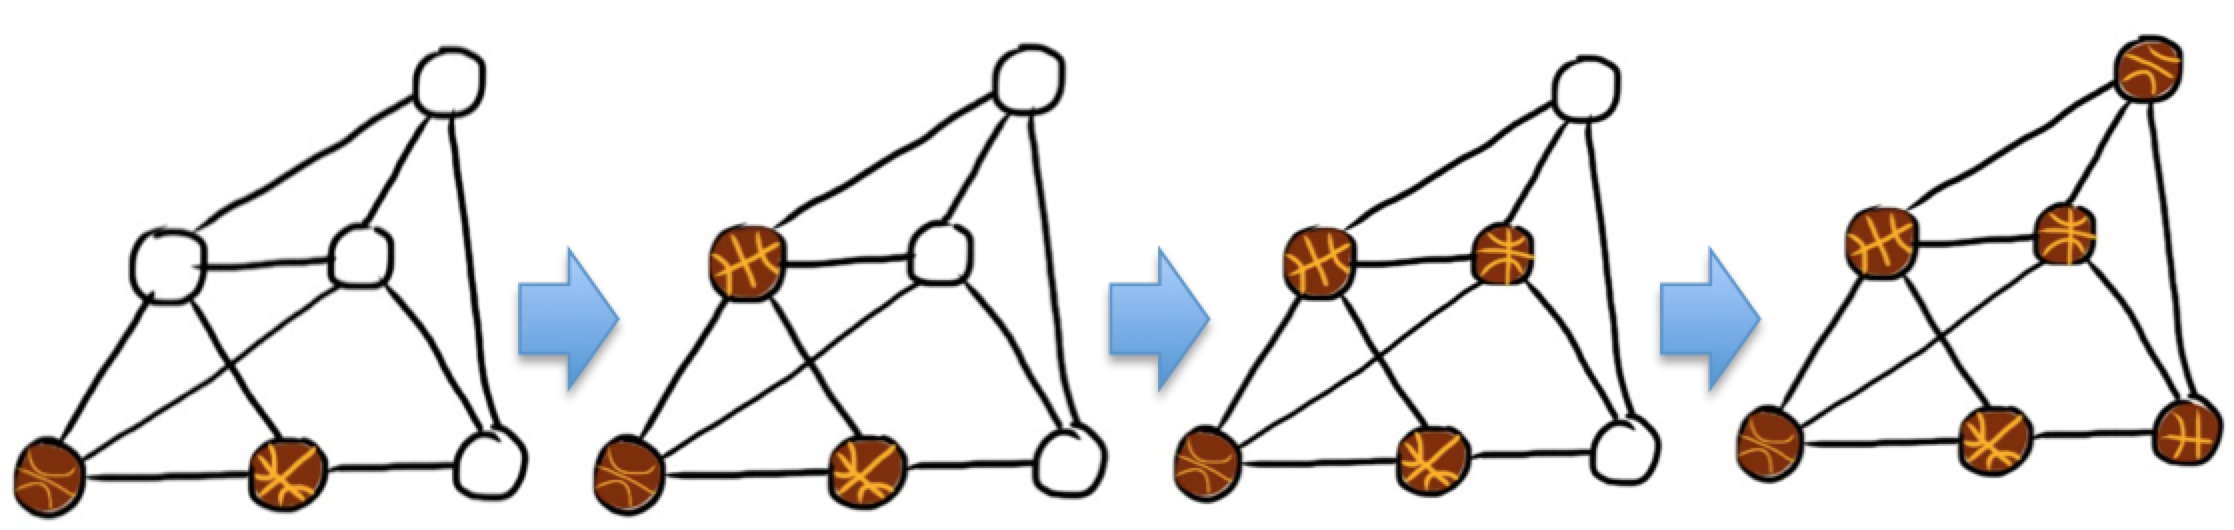
\includegraphics{../images/tema08/coordinacion1.png}
\caption{Juego de coordinación en la que la cascada llega a todos los
nodos (\(q = \frac{2}{5}\))}
\end{figure}

Sin embargo, no podemos suponer que la cascada de adopciones va a llegar
a toda la red (\emph{cascada completa}) sino que hay ocasiones en la que
la cascada se detiene aunque aún hay nodos que siguen manteniendo la
opción B. En el siguiente ejemplo podemos ver que la cascada de
adopciones se detiene tras tres pasos.

\begin{figure}[htbp]
\centering
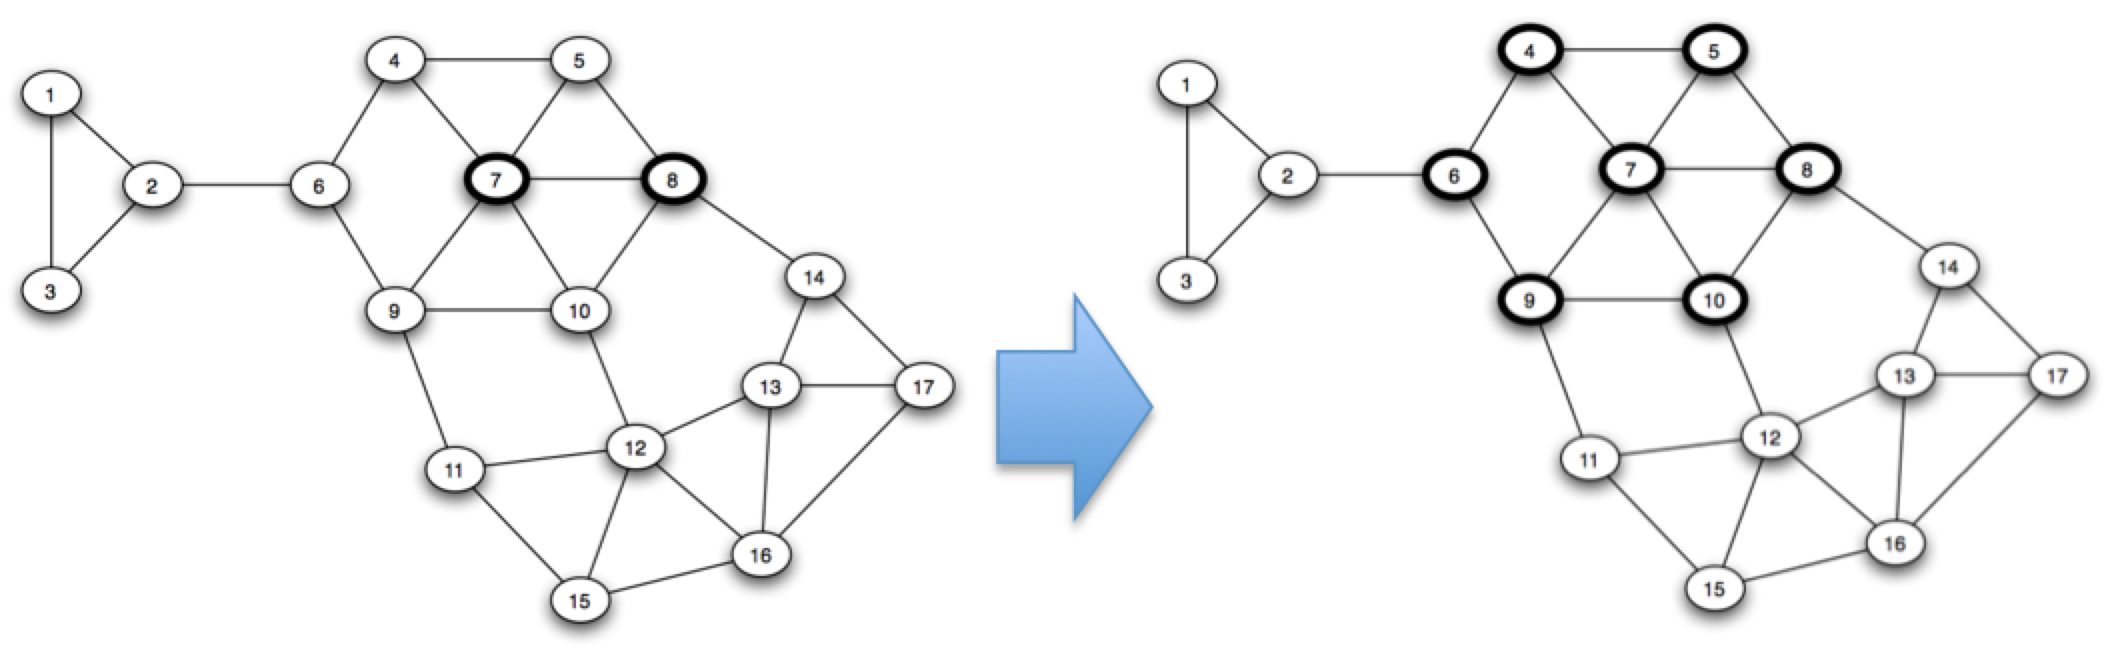
\includegraphics{../images/tema08/coordinacion2.png}
\caption{Juego de coordinación en la que la cascada se detiene tras tres
pasos antes de alcanzar a todos los nodos (\(q = \frac{2}{5}\))}
\end{figure}

Este modelo puede ser utilizado para simular posibles campañas de
marketing viral y ayudar a tomar decisiones en cuanto a qué nodos hay
que influir y cuánto hay que incrementar el beneficio (por ejemplo, la
calidad de un producto) para que se produzca una cascada de difusión
aceptable.

Visto el resultado inicial, la primera opción que se puede tomar es
modificar el beneficio \(a\). En el ejemplo anterior, si aumentamos
\(a =4\) entonces el umbral \(q\) baja a \(q=\frac{1}{3}\) y se puede
ver que la cascada de adopciones alcanza toda la red. De aquí podemos
concluir que la adopción de una nueva opción no solo depende de la
estructura de la red sino que también depende de las diferencias de
beneficios entre la opción A y la opción B.

La segunda opción a tomar, supuesto que no se puede modificar el
beneficio \(a\), está relacionado con decidir a qué nodos de la red es
necesario influir para hacer que la cascada de adopciones alcance al
mayor número posible de nodos en la red. La idea es elegir el menor
número de nodos posible y elegirlos adecuadamente para conseguir que la
cascada se propague. La elección de estos nodos es fundamental en la
cascada de adopciones y está basada intrínsecamente en su posición
dentro de la red.

Si tomamos de nuevo el ejemplo de la red anterior, si mantenemos el
beneficio inicial \(a=3\) y comenzamos la propagación cambiando de
estado a los nodos 12 y 13 entonces conseguiremos que todos los nodos
del 11 al 17 cambien de estado. Sin embargo, si seleccionamos los nodos
11 y 14 entonces no conseguiremos que se propague ningún cambio de
estado por la red.

Podemos ver más en detalle este comportamiento utilizando el
\href{http://www.ladamic.com/netlearn/NetLogo4/DiffusionCompetition.html}{Modelo
de Difusión} que está disponible en la web, seleccionando distintos
nodos iniciales y viendo cómo la propagación se comporta de manera
distinta en unos y otros.

Así mismo, este modelo nos permite comprobar que la estructura de la red
también tiene una fuerte influencia en los procesos de difusión. En
particular, la existencia de comunidades tiene una especial importancia
en los procesos de difusión. Las comunidades tienen tres papeles
fundamentales dentro de estos procesos de difusión:

\begin{itemize}
\itemsep1pt\parskip0pt\parsep0pt
\item
  Las comunidades permiten que se produzca la propagación de los modelos
  basados en umbrales. La existencia de componentes con alta
  conectividad posibilitan la propagación en este tipo de modelos. Sin
  la presencia es ellas no sería posible que se produjese este tipo de
  propagación.
\item
  Las comunidades sirven de barrera para la difusión, de modo que crean
  ``bolsas aisladas'' que no permiten la adopción de ideas externas a la
  comunidad. Cuando una cascada alcanza una comunidad (un agrupamiento
  de nodos de alta densidad) ésta se detendrá ya que no podrá entrar
  dentro de dicha comunidad.
\item
  Lo anterior permite que distintas opiniones puedan convivir en la
  misma red, debido a la existencia de comunidades con distintas
  opiniones en distintos lugares de dicha red.
\end{itemize}

\subsubsection{Otros modelos complejos de
difusión}\label{otros-modelos-complejos-de-difusiuxf3n}

\paragraph*{Nodos bilingües.}\label{nodos-bilinguxfces.}
\addcontentsline{toc}{paragraph}{Nodos bilingües.}

Existen modelos de adopción de opiniones más complejos. Uno de ellos es
el que permite la existencia de \textbf{nodos bilingües}, es decir,
nodos que pueden adoptar la opción A y B simultáneamente pero con una
penalización \(c\).

En este caso, estos nodos pueden conseguir que la opinión minoritaria
persista en la red a pesar en condiciones en las que la opinión
minoritaria desaparecería. A modo de ejemplo podemos utilizar una red
lineal y observar el comportamiento de la misma con y sin nodos
bilingües. Sin ellos, la opción con menor beneficio siempre termina por
desaparecer de la red. Sin embargo, la presencia de nodos bilingües
permite que dicha opción ``sobreviva'' entre pares de estos nodos.
Podemos observar este comportamiento utilizando la simulación del
``Modelo de cascasda'' disponible en el Campus Virtual.

\paragraph*{Umbrales heterogéneos.}\label{umbrales-heteroguxe9neos.}
\addcontentsline{toc}{paragraph}{Umbrales heterogéneos.}

Este modelo considera que cada nodo de la red valora de una manera
diferente las distintas opiniones. De este modo, cada nodo \(v\) de la
red tiene un determinado umbral creado a partir de su beneficio por
adoptar la opción A (\(a_v\)) y su beneficio por adoptar la opción B
(\(b_v\)). La simulación de este modelo funciona de manera similar al
anterior salvo porque cada nodo posee su propio umbral.

En este caso, la diversidad de los umbrales juega un papel muy
importante ya que interactúa de manera compleja con la estructura de la
red. Por ejemplo, en la siguiente figura podemos ver que el nodo 1 tiene
una posición muy central en la red pero que no hubiera tenido éxito en
la propagación de no ser por el bajo umbral del nodo 3. Esto indica que
para comprender la forma en la que se produce la difusión en una red
social no solo hay que tener en cuenta el poder de los influenciadores
sino que también hay que tener en cuenta cómo de influenciables son los
nodos que lo rodean.

\begin{figure}[htbp]
\centering
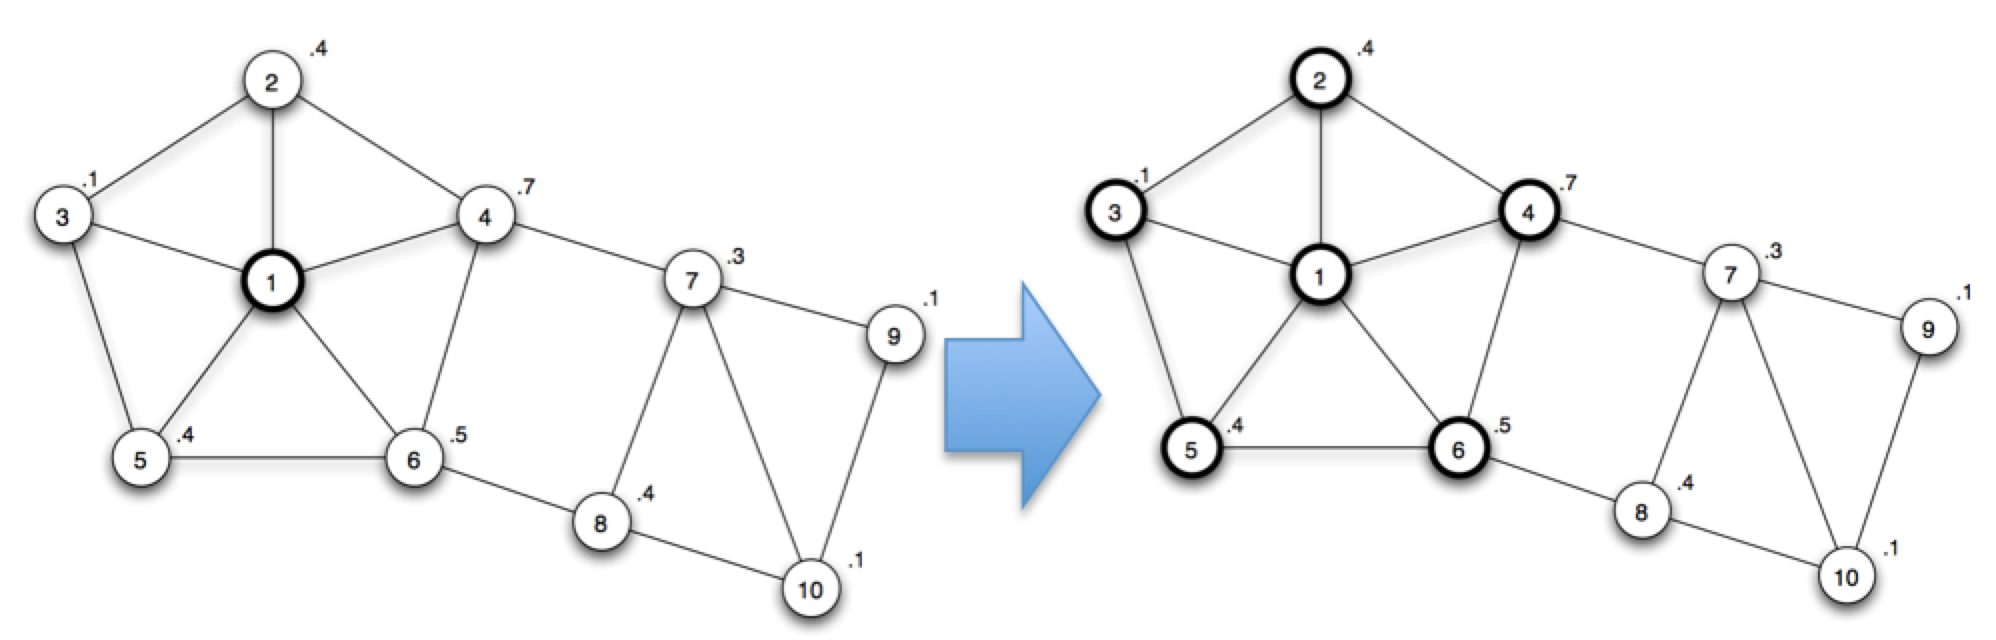
\includegraphics{../images/tema08/umbralHeterogeneo.png}
\caption{Modelo basado en umbrales heterogéneos}
\end{figure}

\paragraph*{Acciones colectivas.}\label{acciones-colectivas.}
\addcontentsline{toc}{paragraph}{Acciones colectivas.}

En esta ocasión lo que se desea es modelar la manera en la que se
coordinan ciertas acciones colectivas como acudir a una manifestación
contra un gobierno represivo. En este caso no tenemos información de las
intenciones del resto de la población (ese gobierno se ha encargado de
controlar los medios de comunicación y hay una ``recompensa'' negativa
por asistir a la manifestación) sino que solo se tiene información de
los individuos más cercanos, lo que dificulta enormemente la toma de
esta decisión. Se produce el fenómeno de lo que se conoce como
\emph{ignorancia pluralista}, en el que no se tiene conocimiento de la
voluntad del resto (aunque realmente haya una verdadera voluntad a favor
o en contra). Este mismo problema de coordinación se puede aplicar en
otras situaciones como los vetos y votaciones de un consejo de
administración o dirección.

La particularidad de este modelo es que pretende predecir el
comportamiento coordinado de una red en el que cada individuo toma la
decisión basándose solo en hablar con las personas más cercanas, es
decir, teniendo un horizonte muy limitado. En general, estas acciones
pueden modelarse mediante un modelo basado en umbrales heterogéneos,
donde el umbral de cada persona significa ``me manifestaré en caso de
que haya al menos \(k\) vecinos en la manifestación (incluyéndome a
mí)''. Así mismo, cada nodo también conoce los umbrales de sus vecinos,
pero no del resto, por lo que es difícil predecir qué ocurrirá. La
decisión se deberá tomar solo usando la información conocida (la suya y
la de sus vecinos).

Por ejemplo, en la siguiente figura se pueden ver tres redes distintas
donde, para cada nodo hemos indicado su umbral. En la primera red no se
producirá la acción colectiva ya que hay un nodo (\(w\)) que tiene un
umbral de 4 y solo hay 3 nodos en la red. En la segunda red, aunque si
todos conociesen la información globalmente se produciría la acción
colectiva, no se producirá dicha acción ya que cada nodo carece de
información suficiente \emph{localmente} para tomar la decisión con
seguridad. En la tercera red existe un conocimiento común: los nodos
\(u\), \(v\) y \(w\) conocen su información y saben que sus vecinos
conocen su información, produciendo una cadena de conocimiento que
permite que los tres nodos realicen la acción colectiva y permitiendo
que también \(x\) la realice.

\begin{figure}[htbp]
\centering
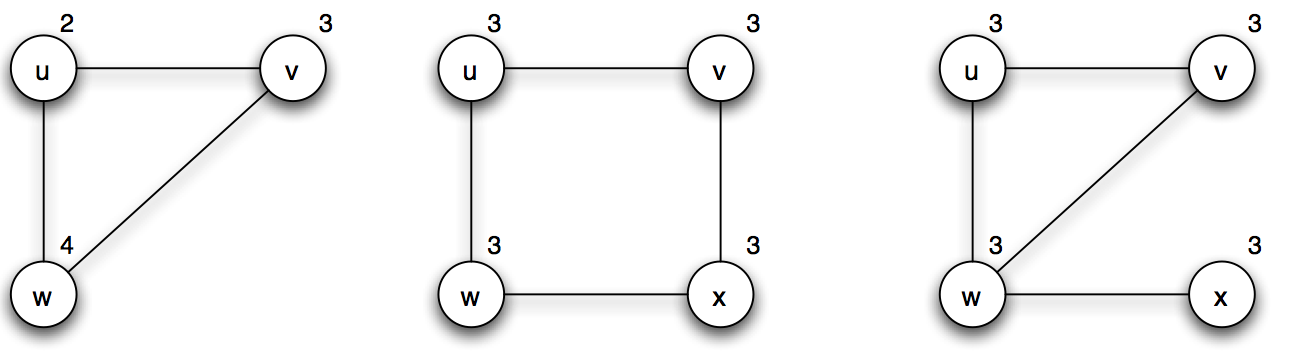
\includegraphics{../images/tema08/accionColectiva.png}
\caption{Modelado de acciones colectivas. Las dos primeras no ocurrirán
mientras que la tercera sí ocurrirá}
\end{figure}

\subsubsection{Difusión de la
innovación}\label{difusiuxf3n-de-la-innovaciuxf3n}

Para concluir con el tema vamos a estudiar un caso muy concreto de
difusión, relacionado con la compartición de información entre personas
para la resolución de problemas y la difusión de la innovación.

Si pretendemos dar solución a un determinado problema podemos pensar en
dos extremos opuestos desde el punto de vista de la comunicación entre
las personas que buscan una solución a dicho problema:

\begin{itemize}
\itemsep1pt\parskip0pt\parsep0pt
\item
  Cada persona trabaja de manera aislada, sin comunicarse con otras
  personas que también trabajan en la resolución del problema. En este
  caso, cualquier solución parcial a la que llegue una de las personas
  no llega al resto de ellas, lo que hace que el avance en la solución
  sea más lento. Sin embargo, esta independencia permite que surjan
  ideas ``frescas'' que no estén sesgadas por el resto de personas que
  trabajan en la búsqueda de una solución.
\item
  Un \emph{brainstorming} o lluvia de ideas es una sesión en la que un
  grupo de personas exponen sus ideas para resolver un problema. En este
  caso, surgen muchas ideas a la vez y unas ideas pueden ayudar a
  mejorar las soluciones propuestas por otros, de modo que se puede
  llegar a una solución de una manera mucho más rápida que de manera
  aislada. Sin embargo, esta interrelación tan fuerte entre estas
  personas puede hacer que todas terminen convergiendo a una idea común
  (\emph{groupthinking}) que no tiene por qué ser la mejor solución al
  problema.
\end{itemize}

Estas dos formas de comunicación las podemos representar en forma de red
tal y como se observa en la siguiente figura.

\begin{figure}[htbp]
\centering
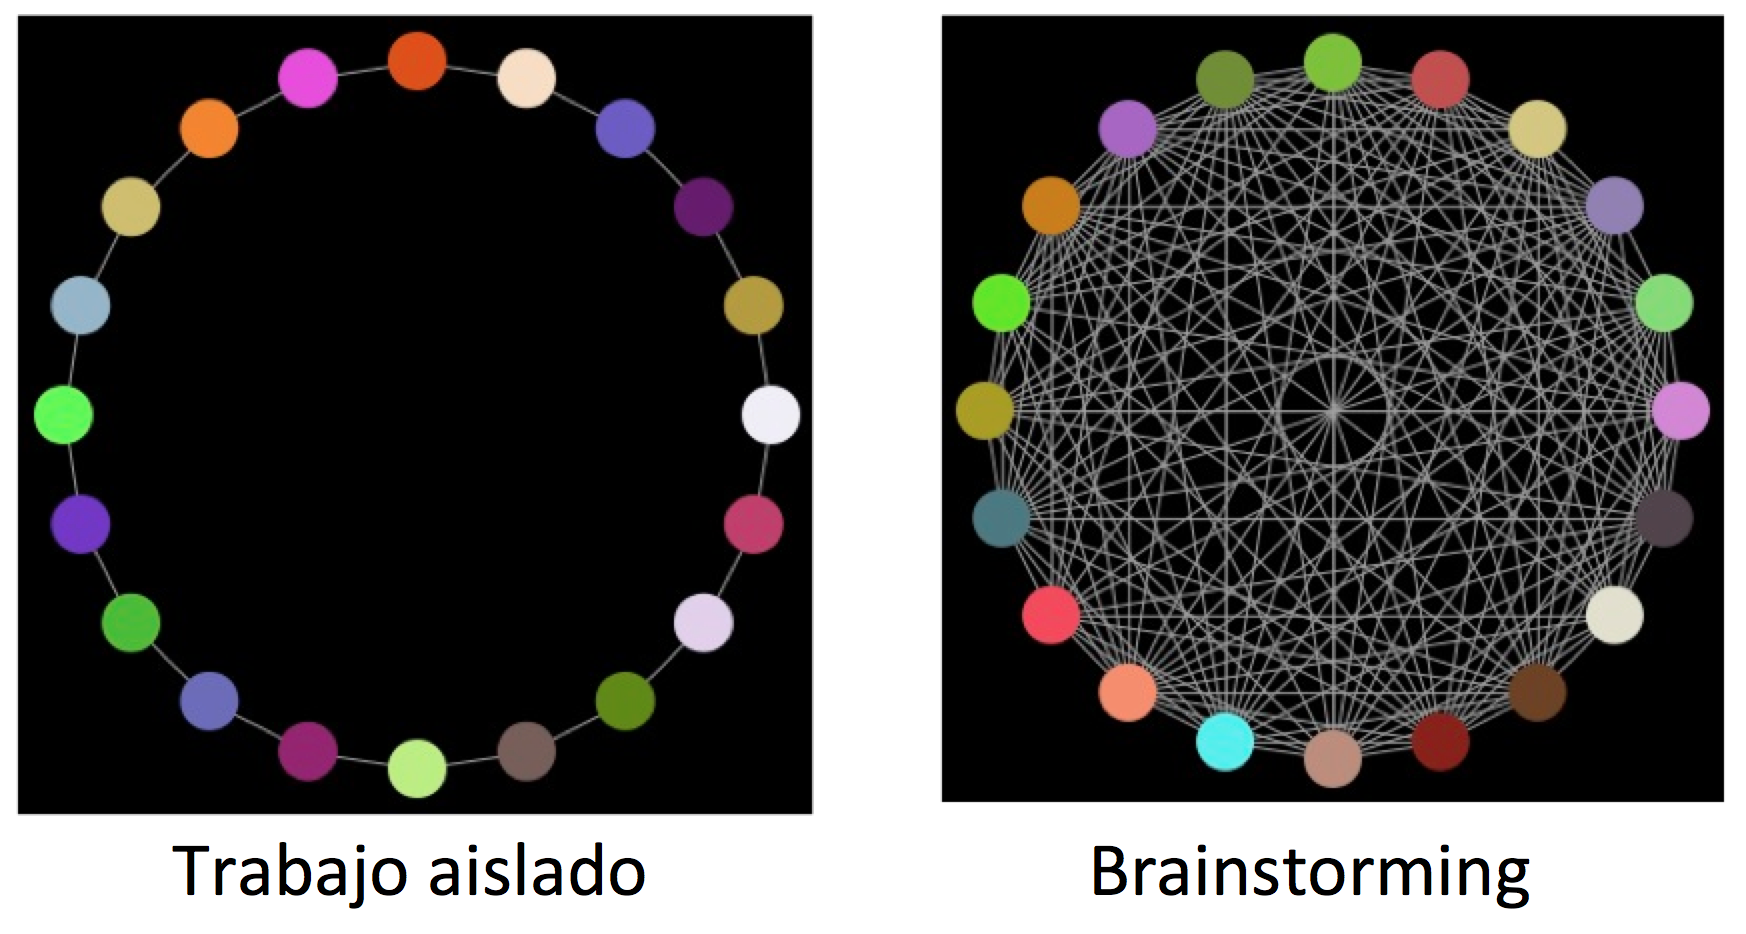
\includegraphics{../images/tema08/redInnovacion.png}
\caption{Redes que representan las dos formas extremas de atacar un
problema}
\end{figure}

Por otro lado, un problema complejo puede quedar representado mediante
su espacio de soluciones, es decir, el conjunto de todas las soluciones
posibles a las que se puede llegar para resolver este problema. De entre
todas las soluciones habrá soluciones mejores y soluciones peores. La
bondad de la solución es calculada mediante una \emph{función de
fitness}, de modo que podemos representar el espacio de soluciones
gráficamente de acuerdo a esta función. Este espacio de soluciones puede
ser más o menos ``rugoso'' dependiendo del problema, es decir, podemos
tener un espacio de soluciones con una única solución buena (la solución
que maximiza la función de fitness) o un espacio donde existan múltiples
máximos locales (soluciones que maximizan la función de fitness en
relación con las soluciones más cercanas). El problema de este segundo
tipo de espacios es que nos podemos quedar en una de estas soluciones
locales sin llegar a conocer que pueden existir soluciones mejores que
la que hemos alcanzado.

Lazer y Friedman usaron el modelo NK de Kauffman\footnote{Lazer, D., \&
  Friedman, A. (2007).
  \href{http://www.ksg.harvard.edu/davidlazer/files/papers/Lazer_Friedman_ASQ.pdf}{The
  network structure of exploration and exploitation}. Administrative
  Science Quarterly, 52(4), 667-694.} para simular el proceso de
difusión de innovación para la resolución de problemas y cómo las red de
comunicación entre las personas implicadas en la resolución del problema
afecta a la velocidad y a la bondad de las soluciones alcanzadas. En
este modelo, \(N\) representa la dimensionalidad del espacio de
soluciones, el número de bits necesarios para representar la solución.
Por ejemplo, en el problema de la mochila\footnote{\href{http://es.wikipedia.org/wiki/Problema_de_la_mochila}{http://es.wikipedia.org/wiki/Problema\emph{de}la\_mochila}},
\(N\) representa cada uno de los objetos que podemos meter en la
mochila, siendo la solución un vector de bits donde 0 representa que no
lo hemos metido en la mochila, mientras 1 representa que sí lo llevamos
en la misma. Por otro lado, \(K\) es un parámetro que mide la rugosidad
del espacio de soluciones. Podemos entender el significado de este
parámetro con la siguiente figura:

\begin{figure}[htbp]
\centering
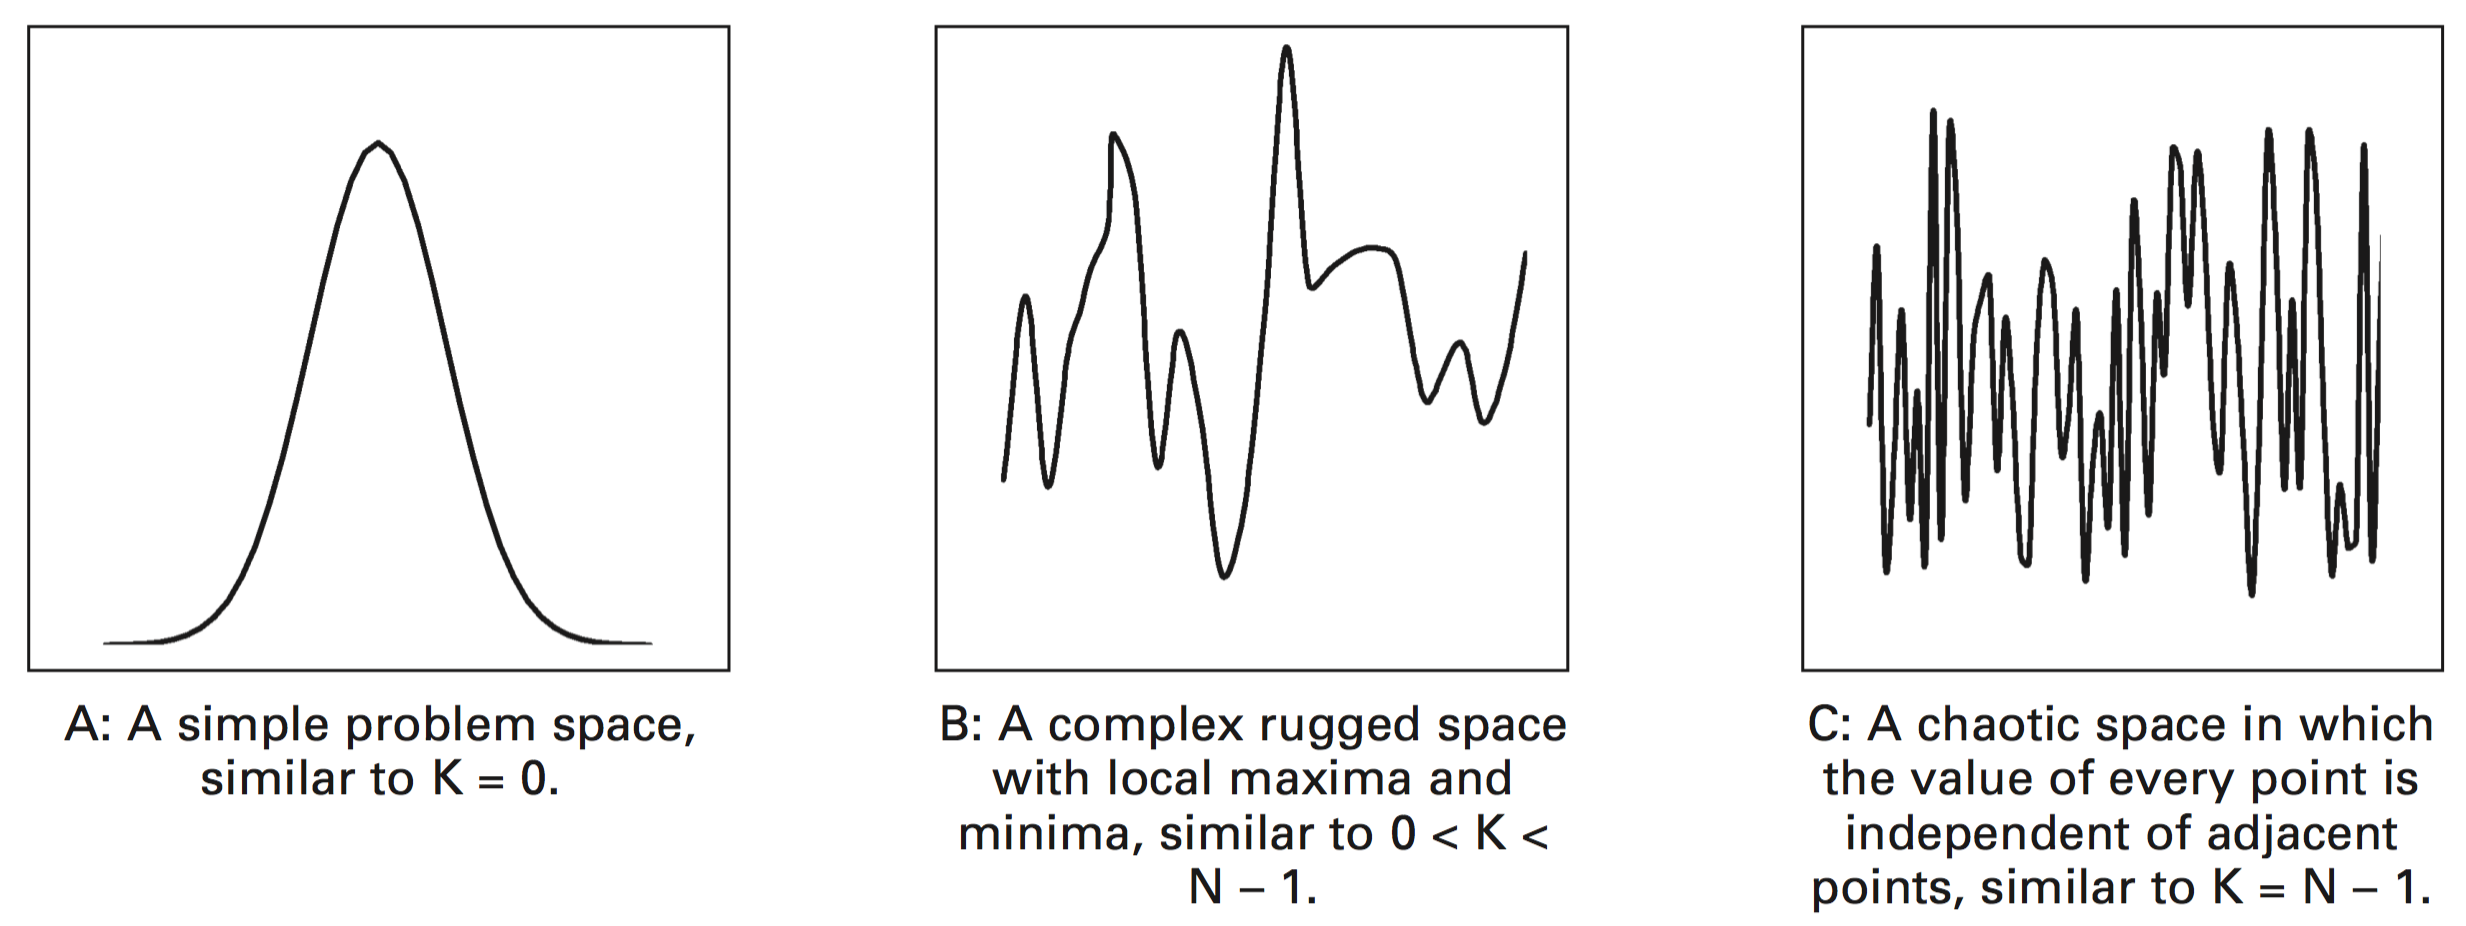
\includegraphics{../images/tema08/NK.png}
\caption{Representación del espacio de soluciones de acuerdo al valor de
\(K\)}
\end{figure}

La simulación del proceso de difusión de innovación consiste en lo
siguiente:

\begin{enumerate}
\def\labelenumi{\arabic{enumi}.}
\itemsep1pt\parskip0pt\parsep0pt
\item
  Tenemos una red en la que cada nodo almacena una cadena de \(N\) bits
  que representa la solución que tiene un determinado individuo de ese
  problema.
\item
  En cada paso de simulación, cada nodo evalúa si alguno de sus vecinos
  tiene una solución mejor que la suya.

  \begin{enumerate}
  \def\labelenumii{\arabic{enumii}.}
  \itemsep1pt\parskip0pt\parsep0pt
  \item
    En caso afirmativo, ``imita'' a su vecino (copia la solución de su
    vecino).
  \item
    En caso negativo, ``innova'', modificando aleatoriamente uno de los
    bits de su solución.
  \end{enumerate}
\item
  La simulación termina cuando todos los nodos convergen a la misma
  solución.
\end{enumerate}

La estructura de la red tiene un fuerte impacto en la velocidad de
difusión de la innovación y cuál es la bondad de la solución alcanzada.
Vamos a probar con una red de mundo pequeño para comprender cómo se
comporta el modelo de difusión. Podemos utilizar el modelo
\href{http://spark-public.s3.amazonaws.com/sna/netlearn/NetLogo502/SmallWorldInnovation.html}{SmallWorld
Innovation}, disponible en el Campus Virtual.

Las conclusiones que se obtienen de esta simulación es que cuanto mayor
es la comunicación entre los nodos más rápido se converge a una solución
mejor que la media inicial. Sin embargo, esta solución no es tan buena
como la que se alcanza en una red con menos conexiones ya que no ha
habido suficiente tiempo como para que la innovación se propague por la
red. La red con menos conexiones alcanza una solución mejor pero, por
contra, tarda más en converger.

\begin{figure}[htbp]
\centering
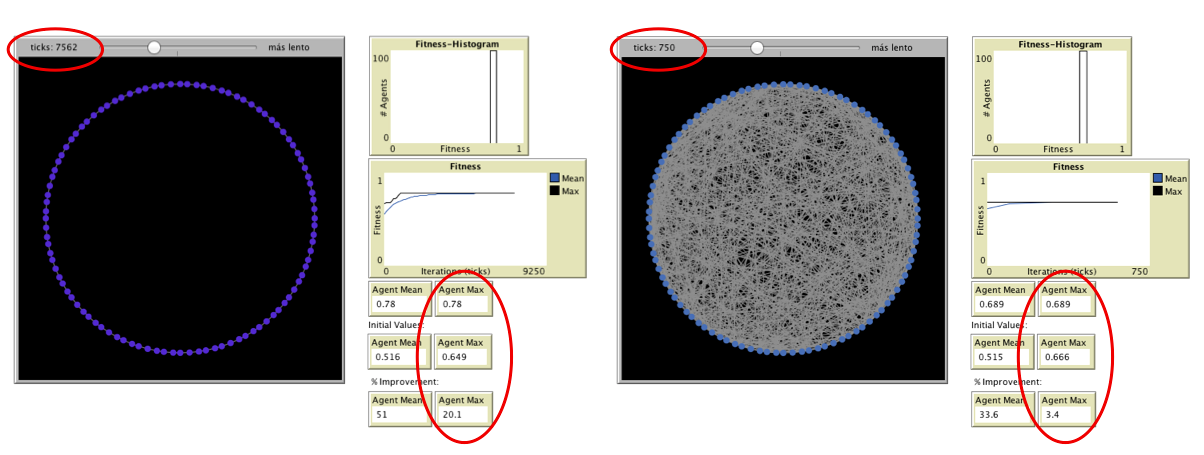
\includegraphics{../images/tema08/solSimulacion.png}
\caption{Solucioones finales que alcanza la simulación. La red de la
izquierda converge a una solución mejor pero tarda mucho más tiempo.}
\end{figure}

\end{document}
